%%%%%%%%%%%%%%%%%%%%%%%%%%%%%%%%%%%%%%%%%
% Masters/Doctoral Thesis 
% LaTeX Template
% Version 1.43 (17/5/14)
%
% This template has been downloaded from:
% http://www.LaTeXTemplates.com
%
% Original authors:
% Steven Gunn 
% http://users.ecs.soton.ac.uk/srg/softwaretools/document/templates/
% and
% Sunil Patel
% http://www.sunilpatel.co.uk/thesis-template/
%
% License:
% CC BY-NC-SA 3.0 (http://creativecommons.org/licenses/by-nc-sa/3.0/)
%
% Note:
% Make sure to edit document variables in the Thesis.cls file
%
%%%%%%%%%%%%%%%%%%%%%%%%%%%%%%%%%%%%%%%%%

%----------------------------------------------------------------------------------------
%	PACKAGES AND OTHER DOCUMENT CONFIGURATIONS
%----------------------------------------------------------------------------------------

\documentclass[11pt, oneside]{Report} % The default font size and one-sided printing (no margin offsets)

\graphicspath{{Pictures/}} % Specifies the directory where pictures are stored

\usepackage[square, numbers, comma, sort&compress]{natbib} % Use the natbib reference package - read up on this to edit the reference style; if you want text (e.g. Smith et al., 2012) for the in-text references (instead of numbers), remove 'numbers' 
\usepackage{adjustbox}
\hypersetup{urlcolor=blue, colorlinks=true} % Colors hyperlinks in blue - change to black if annoying
\title{\ttitle} % Defines the thesis title - don't touch this
\usepackage{float}
\begin{document}

\frontmatter % Use roman page numbering style (i, ii, iii, iv...) for the pre-content pages

\setstretch{1.3} % Line spacing of 1.3

% Define the page headers using the FancyHdr package and set up for one-sided printing
\fancyhead{} % Clears all page headers and footers
\rhead{\thepage} % Sets the right side header to show the page number
\lhead{} % Clears the left side page header

\pagestyle{fancy} % Finally, use the "fancy" page style to implement the FancyHdr headers

\newcommand{\HRule}{\rule{\linewidth}{0.5mm}} % New command to make the lines in the title page

% PDF meta-data
\hypersetup{pdftitle={\ttitle}}
\hypersetup{pdfsubject=\subjectname}
\hypersetup{pdfauthor=\authornames}
\hypersetup{pdfkeywords=\keywordnames}

\makeatletter
\def\@makechapterhead#1{%
  \vspace*{50\p@}%
  {\parindent \z@ \raggedright \normalfont
    \ifnum \c@secnumdepth >\m@ne
      \if@mainmatter
        %\huge\bfseries \@chapapp\space \thechapter
        \Huge\bfseries \thechapter.\space%
        %\par\nobreak
        %\vskip 20\p@
      \fi
    \fi
    \interlinepenalty\@M
    \Huge \bfseries #1\par\nobreak
    \vskip 40\p@
  }}
\makeatother

%----------------------------------------------------------------------------------------
%	TITLE PAGE
%----------------------------------------------------------------------------------------

\begin{titlepage}
\begin{center}
	\begin{minipage}[t]{0.48\textwidth}
	  \begin{flushleft}
	    \includegraphics [width=40mm]{Logo} 
	  \end{flushleft}
	\end{minipage}
	\begin{minipage}[t]{0.48\textwidth}
	  \begin{flushright}
	  \end{flushright}
	\end{minipage} \\[2cm]
	
\textsc{\Large Livrable de Projet}\\[0.5cm] % Thesis type

\HRule \\[0.4cm] % Horizontal line
{\huge \bfseries \ttitle}\\[0.4cm] % Thesis title
\HRule \\[1.5cm] % Horizontal line
 
\begin{minipage}[t]{0.4\textwidth}
\begin{flushleft} \large
\emph{Hexanôme \textbf{H4303}}\\
{\authornames}
\end{flushleft}
\end{minipage}
\begin{minipage}[t]{0.48\textwidth}
\begin{flushright} \large
\emph{Enseignants} \\
{\supname}
\end{flushright}
\end{minipage}\\[3cm]
{\large \today}\\[4cm] % Date

\vfill
\footnotesize{Année scolaire 2014-2015}
\end{center}

\end{titlepage}



%----------------------------------------------------------------------------------------
%	LIST OF CONTENTS/FIGURES/TABLES PAGES
%----------------------------------------------------------------------------------------

\pagestyle{fancy} % The page style headers have been "empty" all this time, now use the "fancy" headers as defined before to bring them back

\lhead{\emph{Table des matières}} % Set the left side page header to "Contents"
\tableofcontents % Write out the Table of Contents

\lhead{\emph{Figures}} % Set the left side page header to "List of Figures"
\listoffigures % Write out the List of Figures

\lhead{\emph{Tables}} % Set the left side page header to "List of Tables"
\listoftables % Write out the List of Tables


%----------------------------------------------------------------------------------------
%	CONTENT - CHAPTERS
%----------------------------------------------------------------------------------------
\mainmatter % Begin numeric (1,2,3...) page numbering

\pagestyle{fancy} % Return the page headers back to the "fancy" style
\chapter*{Introduction}
\addcontentsline{toc}{chapter}{Introduction}

Ce dossier vise à vous présenter le système de gestion des livraisons commandé par le Grand Lyon au service des entreprises de transport afin de minimiser le nombre de camions qui circulent en ville.

Nous allons nous intéresser en particulier au sous-système "Préparation et supervisions des livraisons", permettant aux superviseurs de préparer les tournées du lendemain, de modifier ces tournées et de superviser l'ensemble des livraisons de la journée.
% Chapter Template

\chapter{Capture et analyse des besoins} % Main chapter title

\label{Chapter1} % Change X to a consecutive number; for referencing this chapter elsewhere, use \ref{ChapterX}

\lhead{Chapter 1. \emph{Capture et analyse des besoins}} % Change X to a consecutive number; this is for the header on each page - perhaps a shortened title

%----------------------------------------------------------------------------------------
%	SECTION 1
%----------------------------------------------------------------------------------------

\section{Planning prévisionnel du projet}
\begin{figure}[htbp]
	\centering
		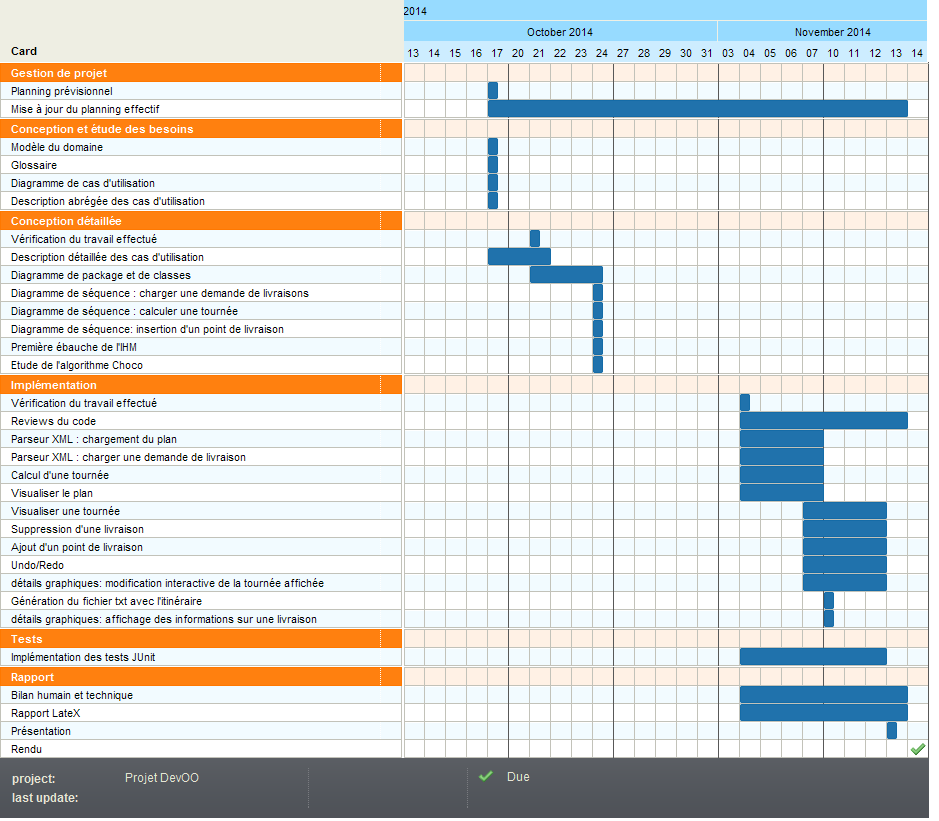
\includegraphics[width=\textwidth,height=\textheight,keepaspectratio]{Figures/previsional_plan}
		\rule{35em}{0.5pt}
	\caption[Planning prévisionnel]{Planning prévisionnel du projet}
\end{figure}

%----------------------------------------------------------------------------------------
%	SECTION 2
%----------------------------------------------------------------------------------------

\section{Modèle du domaine}

\begin{figure}[H]
	\centering
		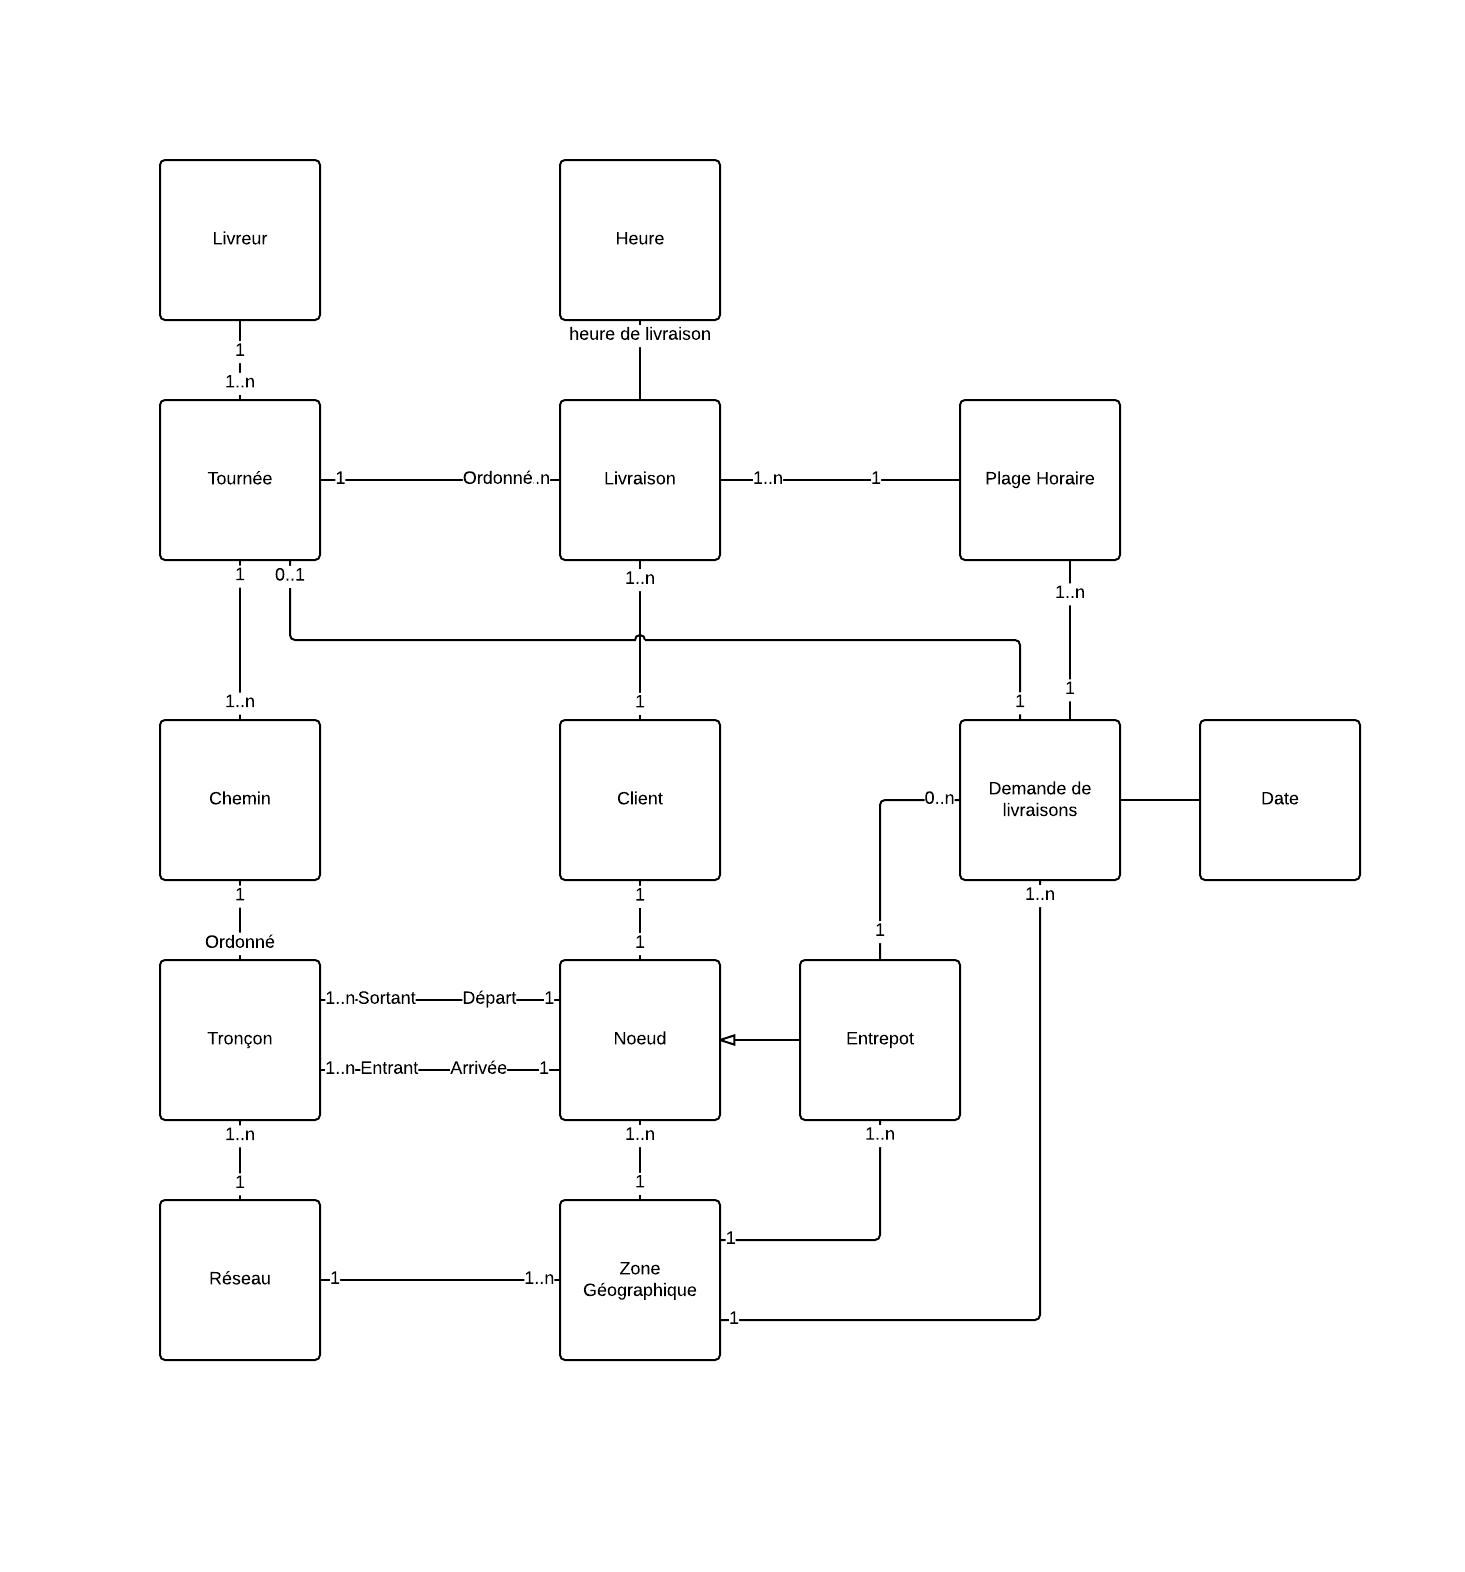
\includegraphics[width=\textwidth,height=\textheight,keepaspectratio]{Figures/modele_domaine}
		\rule{35em}{0.5pt}
	\caption[Modèle du domaine]{Modèle du domaine}
\end{figure}
\clearpage

\section{Diagramme de cas d'utilisation}
\begin{figure}[htbp]
	\centering
		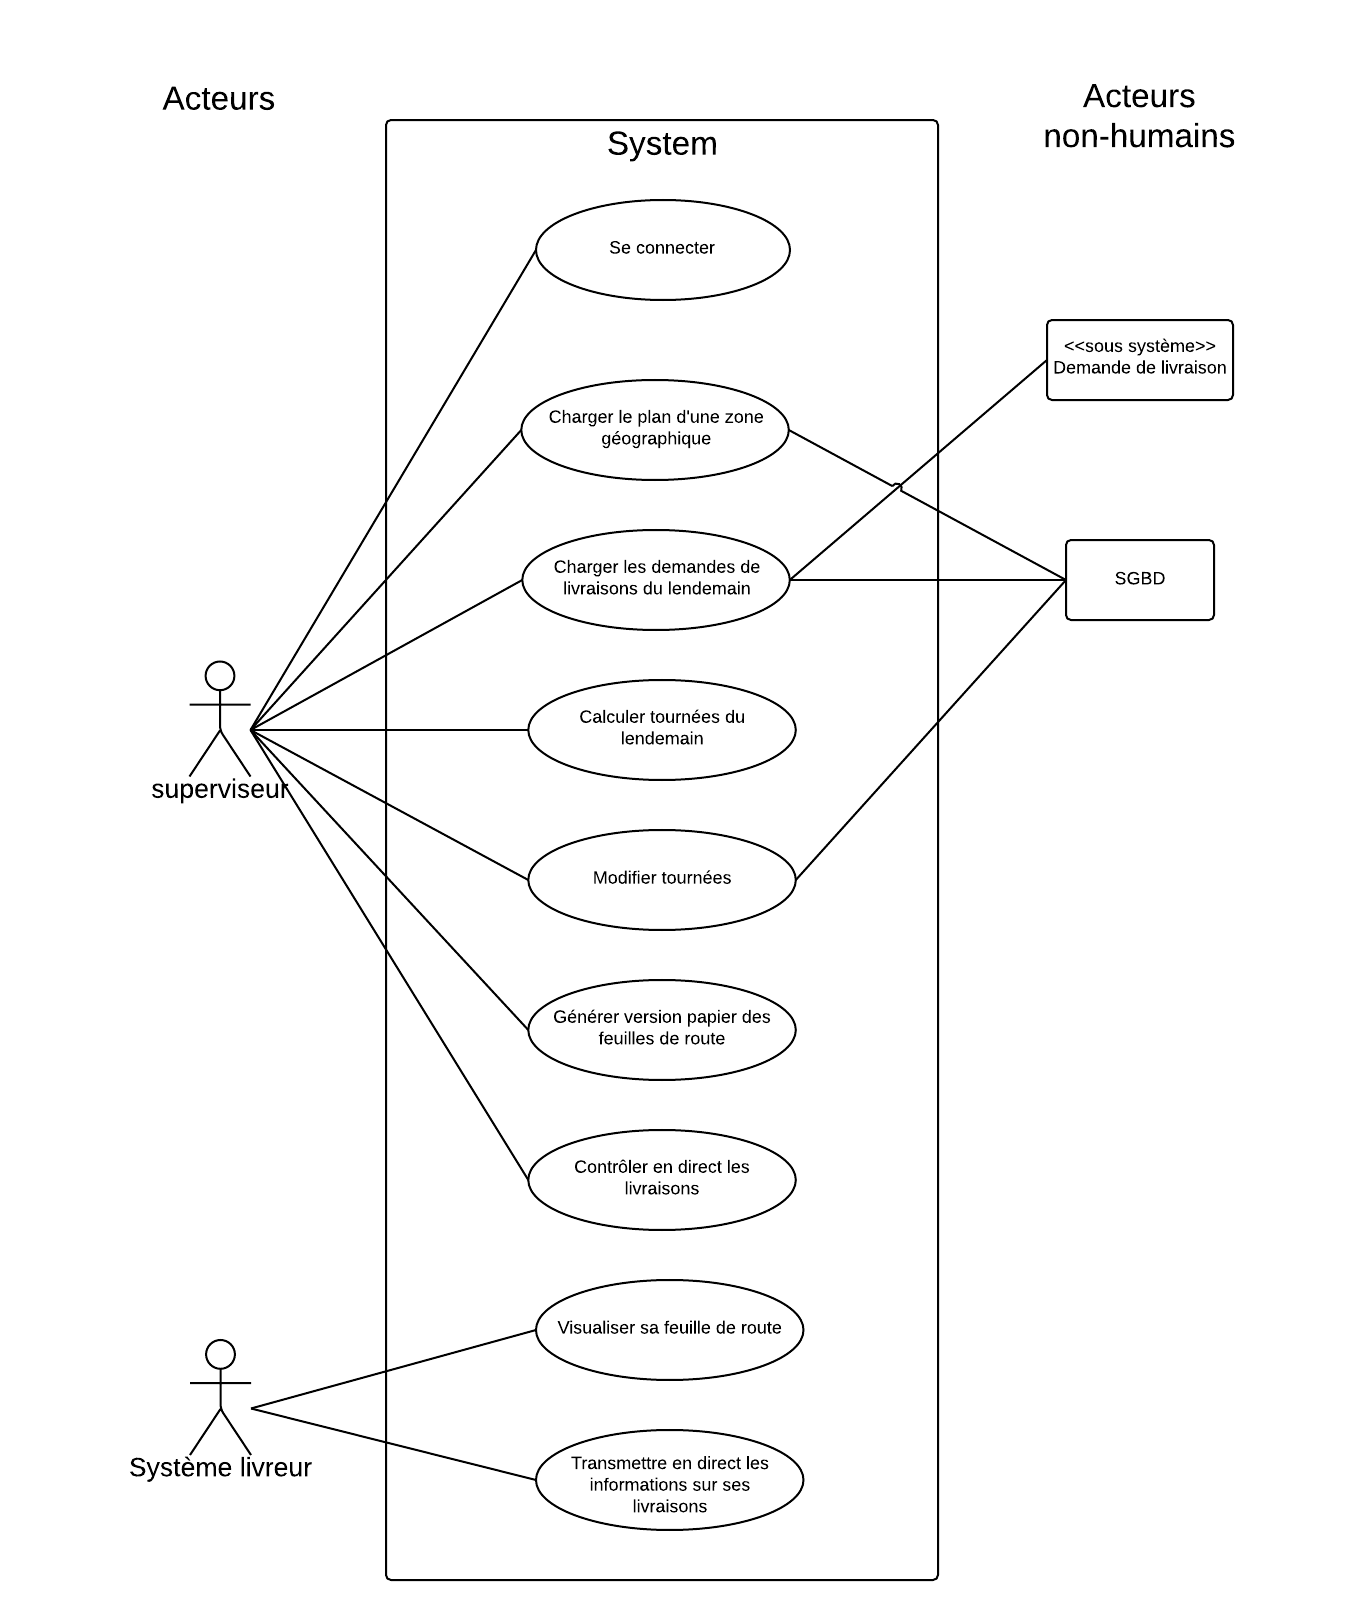
\includegraphics[width=\textwidth,height=\textheight,keepaspectratio]{Figures/cu}
		\rule{35em}{0.5pt}
	\caption[Planning prévisionnel]{Planning prévisionnel du projet}
\end{figure}
\section{Description textuelle abrégée des cas d'utilisation}
\subsection{Superviseur}
\begin{description}
\item [Se connecter au Système]Le Superviseur rentre son identifiant et son mot de passe pour se connecter.
\item [Charger le plan d’une zone géographique]Le Superviseur fournit au Système le plan de la zone géographique voulue. Le Système valide la saisie du plan.
\item [Charger les demandes de livraison du lendemain]Le sous-système “Demande de livraison” fournit au Système les demandes de livraison du lendemain. Le Système valide la bonne réception et la cohérence des données. 
\item [Calculer les tournées du lendemain]En se basant sur la plan de la zone et les demandes de livraison, le Système calcule les tournées du lendemain. Le Système affiche les tournées au Superviseur et les éventuels problèmes (plages horaires non respectées).
\item [Modifier tournées (avant validation)]Le Superviseur résout les éventuels problèmes en contactant les clients concernés et en modifiant manuellement les tournées en plaçant considérant le ou les nouveaux points et en supprimant l’ancien qui posait problème. Cette suppression entraînant une cassure entre deux points, le Système calcule le plus court chemin entre ces deux points.
\item [Générer version papier des feuilles de route] Le Superviseur valide les tournées puis imprime les feuilles de route (version papier).
\item [Contrôler les livraisons en direct] Le Superviseur consulte le Système pour obtenir les informations sur les livraisons effectuées ou non-effectuées. Ces informations proviennent du Système Livreur qui renvoie les données des livraisons en cours.
Le Superviseur peut modifier interactivement les tournées.
\end{description}
\subsection{Système livreur}
\begin{description}
\item [Visualiser sa feuille de route]Le Système Livreur consulte en direct sa tournée, mise à jour en temps réel avec le Système, car le Superviseur peut la modifier en direct.
\item [Transmettre en direct les informations sur les livraisons]A chaque livraison le Système Livreur envoie un message de confirmation au Système. Si la livraison n’a pas pu être effectuée, le Système Livreur envoie tout de même un message au Système pour signaler son échec.


\end{description}
% Chapter Template

\chapter{Conception} % Main chapter title

\label{Chapter2} % Change X to a consecutive number; for referencing this chapter elsewhere, use \ref{ChapterX}

\lhead{Chapitre 2. \emph{Conception}} % Change X to a consecutive number; this is for the header on each page - perhaps a shortened title

%----------------------------------------------------------------------------------------
%	SECTION 1
%----------------------------------------------------------------------------------------

\section{Description textuelle structurée des cas d'utilisation}

%-----------------------------------
%	SUBSECTION 1
%-----------------------------------
\subsection{Se connecter au système}
\begin{enumerate}
\item Scénario de base 
\begin{enumerate}
\item Le Superviseur se connecte, en tant que tel, en remplissant le formulaire de connexion présent sur la page d’accueil puis en cliquant sur le bouton “Se connecter”.

\end{enumerate}
\item Extensions
\begin{enumerate}
\item Erreur de connexion

\begin{enumerate}
\item Message d’erreur et retour à l’étape 1 du scénario de base.
\end{enumerate}
\end{enumerate}
\end{enumerate}

\subsection{Charger le plan d'une zone}
\begin{enumerate}
\item Précondition
\begin{enumerate}
\item 
Se connecter au Système
\end{enumerate}


\item Scénario de base
\begin{enumerate}
\item Erreur de connexion
\item Le Système indique le niveau de chargement du fichier grâce à une petite icône de chargement.
\item Le Système valide la conformité du fichier en affichant une icône de validation verte.
\item Le système affiche le plan chargé dans l’espace prévu
\end{enumerate}

\item Extensions
\begin{description}
\item [Chargement interrompu] Le Système indique l’échec du chargement : croix rouge + message d’erreur : ”Erreur de chargement du fichier, veuillez recommencer”
\item [Fichier incorrect : erreur rédhibitoire] Traitement interrompu et affichage d’erreur :  croix rouge accompagnée du message d’erreur correspondant.
\item [Fichier incorrect : erreur acceptable]
Le traitement du fichier continue mais un message explique l’erreur et en conséquence ce qui n’a pas été chargé 
\end{description}
\end{enumerate}

%-----------------------------------
%	SUBSECTION 2
%-----------------------------------

\subsection{Charger et calculer une demande de livraisons}
\begin{enumerate}
\item Précondition
\begin{enumerate}
\item Se connecter au Système + Charger plan d’une zone géographique
\end{enumerate}


\item Scénario de base
\begin{enumerate}
\item Le Superviseur clique sur le menu Fichier puis le sous-menu “Charger les demandes de livraison” puis va chercher le fichier correspondant.  
\item Le Système indique le niveau de chargement du fichier grâce à une petite icône de chargement.
\item Le Système valide la conformité du fichier en affichant une icône de validation verte.
\item Le système met à jour l’affichage du plan avec une première proposition de chemin ?
\item Le Système affiche plusieurs nouvelles sections. Une section plan contenant les tournées, des boutons “annuler”, “refaire”, zoom “+” et dézoom “-”.  Une section “Information sur le noeud sélectionné” contenant au départ un texte : “Cliquez sur un point de livraison pour afficher ses informations” et une section ayant le bouton “Générer la feuille de route”.

\end{enumerate}

\item Extensions
\begin{description}
\item [Chargement interrompu] Le Système indique l’échec du chargement : croix rouge + message d’erreur :”Erreur de chargement, veuillez recommencer”.
\item [Fichier incorrect : erreur rédhibitoire] Traitement interrompu et affichage d’erreur :  croix rouge accompagnée du message d’erreur correspondant.
\item [Fichier incorrect : erreur acceptable] Le traitement du fichier continue mais un message explique l’erreur et en conséquence ce qui n’a pas été chargé.
\item [Une tournée calculée contient des problèmes] Le Système indique le problème par un point d'exclamation sur le plan, au niveau du point correspondant.
\end{description}
\end{enumerate}

\subsection{Modifier une tournée la veille}
\begin{enumerate}
\item Précondition
\begin{enumerate}
\item Se connecter au Système + Charger plan d’une zone géographique + Charger et calculer les demandes de livraison du lendemain
\end{enumerate}

\item Scénario de base : Suppression d'un point
\begin{enumerate}
\item Le Superviseur clique sur un point de livraison de la tournée puis clique sur le bouton “Supprimer”.
\item Le Système calcule le chemin le plus court entre les points précédent et suivant du point supprimé.
\item Le Système met à jour l’affichage du plan.
\item Le Système dégrise le bouton Annuler qui est dans le menu Édition.

\end{enumerate}

\item Scénario de base : Insertion d'un point
\begin{enumerate}
\item Le Superviseur clique sur un nœud.
\item Le Système affiche “Cliquez sur le point suivant votre nouveau point de livraison”.
\item Le Superviseur clique le point suivant le nouveau point de livraison.
Le Système calcule le chemin le plus court entre le point ajouté et le point le précédent puis entre le point ajouté et le point le suivant.
\item Le Système met à jour l’affichage du plan.
\item Le Système dégrise le bouton Annuler qui est dans le menu Édition

\end{enumerate}
\item Extensions
\begin{enumerate}
\item Le Superviseur clique que sur un nœud mais ne clique pas ensuite sur un point de livraison.
\begin{enumerate}
\item Le nœud ne devient pas un point de livraison.
\end{enumerate}
\end{enumerate}
\end{enumerate}

\subsection{Annuler des modifications}
\begin{enumerate}
\item Précondition
\begin{enumerate}
\item Avoir modifié au moins une fois la tournée, avoir fini un des scénarios de base.
\end{enumerate}


\item Scénario de base : Annuler insertion
\begin{enumerate}
\item Le Superviseur clique sur le menu Edition puis le sous-menu “Annuler”.
\item Le Système supprime le point dernièrement crée.
\item Le Système met à jour l’affichage du plan.
\item Le Système grise le bouton Annuler si il n’y a plus d’actions à annuler.


\end{enumerate}
\item Scénario de base : Annuler suppression
\begin{enumerate}
\item Le Système recrée le point dernièrement supprimer et recalcule la tournée.
\item Le Système met à jour l’affichage du plan.
\item Le Système grise le bouton Annuler si il n’y a plus d’actions à annuler.
\end{enumerate}
\end{enumerate}




\subsection{Refaire des modifications}
\begin{enumerate}
\item Précondition
\begin{enumerate}
\item Avoir annulé une opération.
\end{enumerate}


\item Scénario de base : Annuler dernière opération

\end{enumerate}
\subsection{Générer une feuille de route}

\begin{enumerate}
\item Précondition
\begin{enumerate}
\item Se connecter au Système + Charger plan d’une zone géographique + Charger les demandes de livraison du lendemain + Générer une tournée

\end{enumerate}


\item Scénario de base 
\begin{enumerate}
\item Le Superviseur clique sur le bouton “Générer la feuille de route”.
\item Le Système édite une version txt de l’ensemble des feuilles de route. 
\end{enumerate}
\end{enumerate}




%----------------------------------------------------------------------------------------
%	SECTION 2
%----------------------------------------------------------------------------------------
\clearpage
\section{Diagrammes de packages et de classes}
\subsection{Package model}
\begin{figure}[H]
\centering
	\centering
		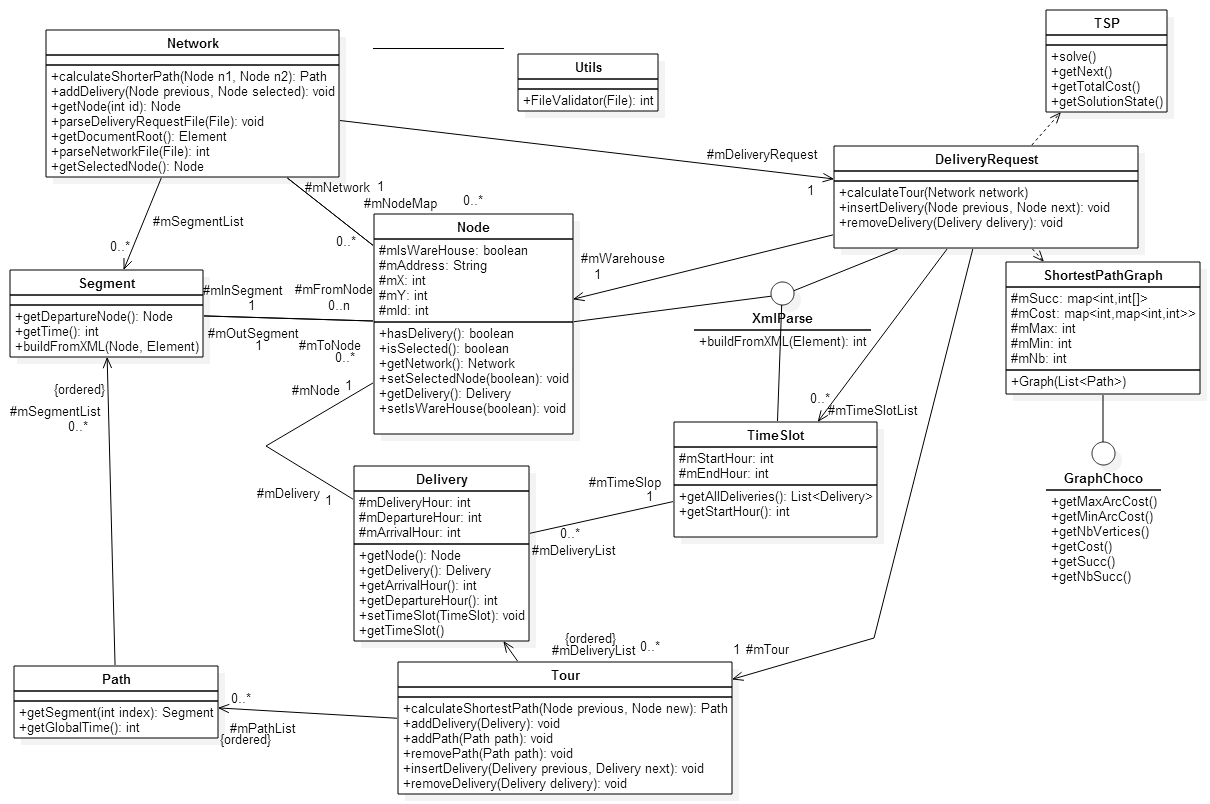
\includegraphics[width=\textwidth,height=\textheight,keepaspectratio, angle=90]{Figures/modele}
		\rule{35em}{0.5pt}
	\caption[Model]{Package Model}
\end{figure}

\subsection{Package view}
\begin{figure}[H]
	\centering
		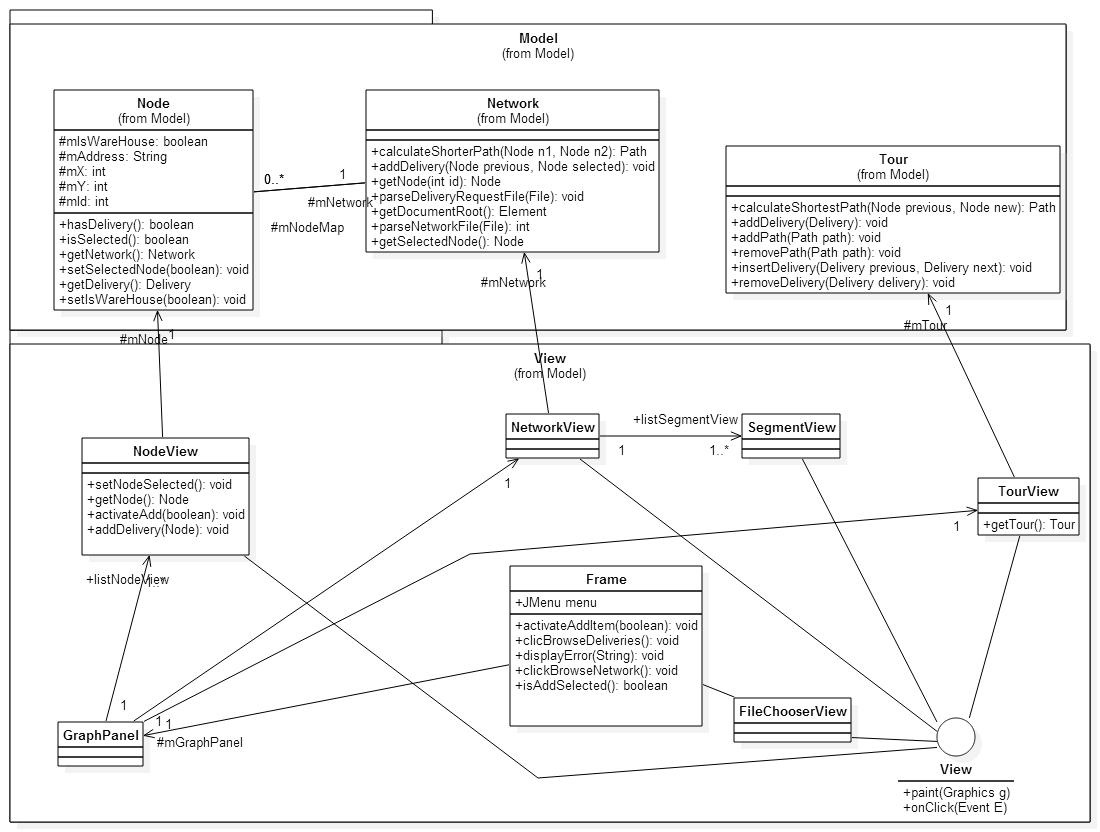
\includegraphics[width=\textwidth,height=\textheight,keepaspectratio, angle=90]{Figures/vue}
		\rule{35em}{0.5pt}
	\caption[View]{Package View}
\end{figure}

\subsection{Package controller}
\begin{figure}[H]
	\centering
		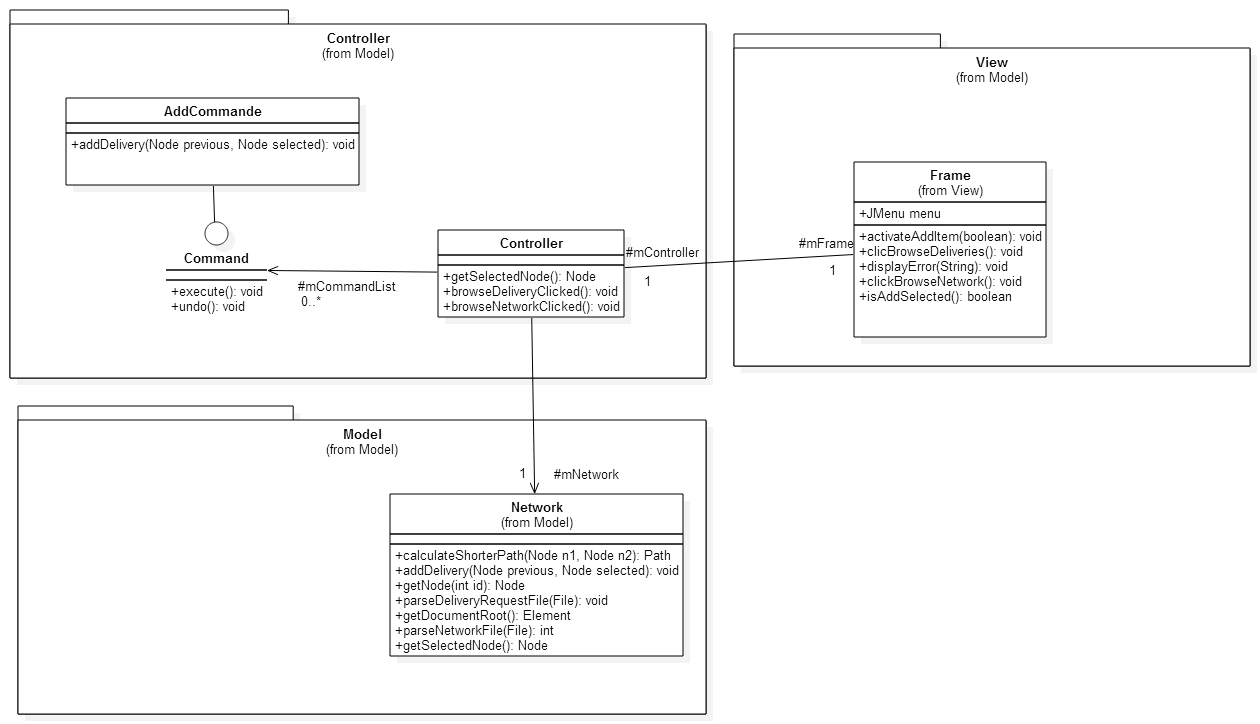
\includegraphics[width=\textwidth,height=\textheight,keepaspectratio, angle=90]{Figures/controleur}
		\rule{35em}{0.5pt}
	\caption[Controller]{Package Controller}
\end{figure}


\section{Diagrammes de séquence}

\subsection{Chargement du plan d'une zone}
\begin{figure}[H]
	\centering
		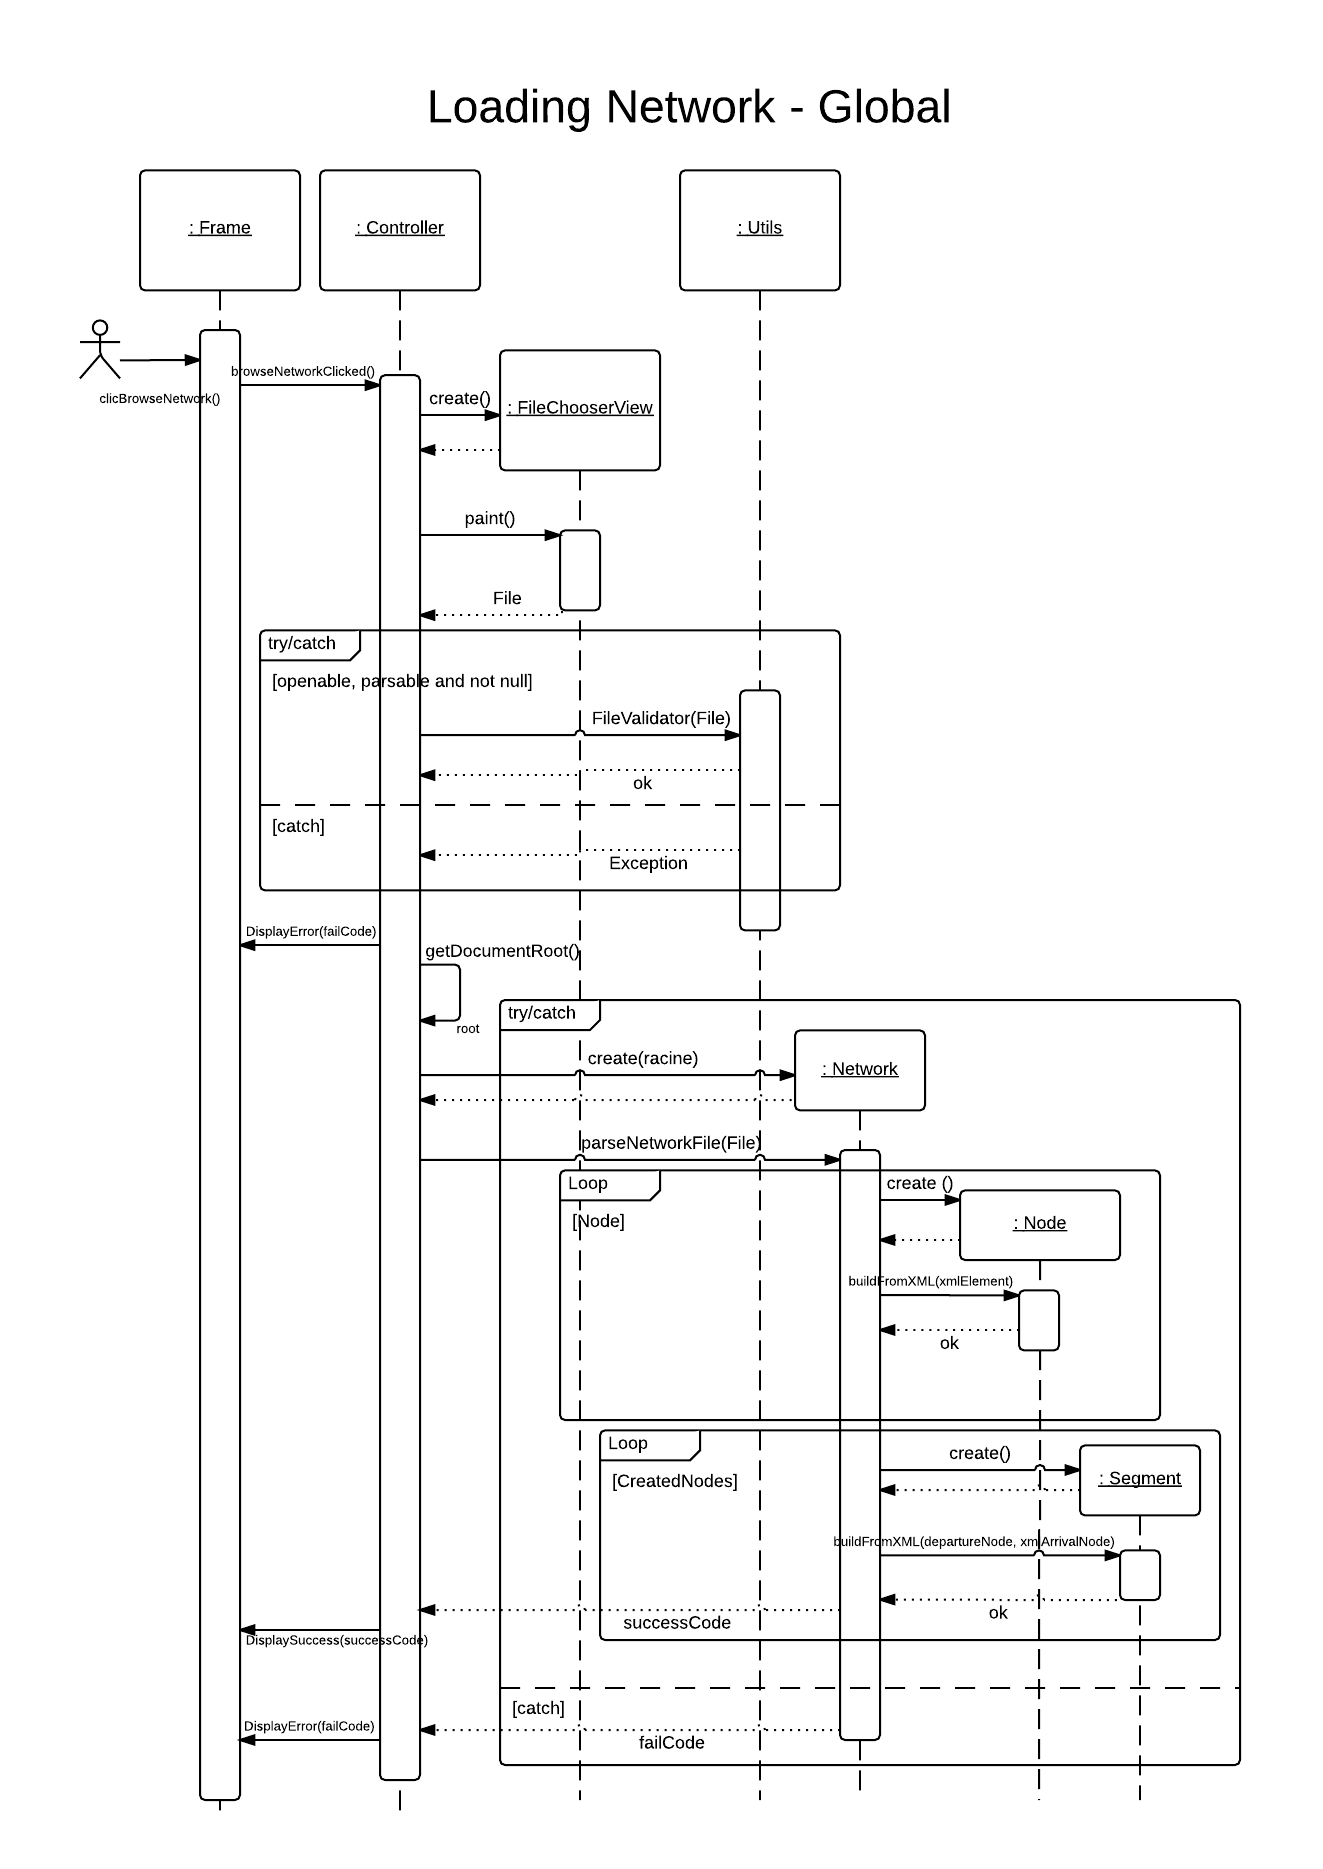
\includegraphics[width=\textwidth,height=\textheight,keepaspectratio]{Figures/plan_zone}
		\rule{35em}{0.5pt}
	\caption[Chargement du plan d'une zone]{Chargement du plan d'une zone}
\end{figure}

\subsection{Chargement d'une demande de livraison}
\begin{figure}[H]
	\centering
		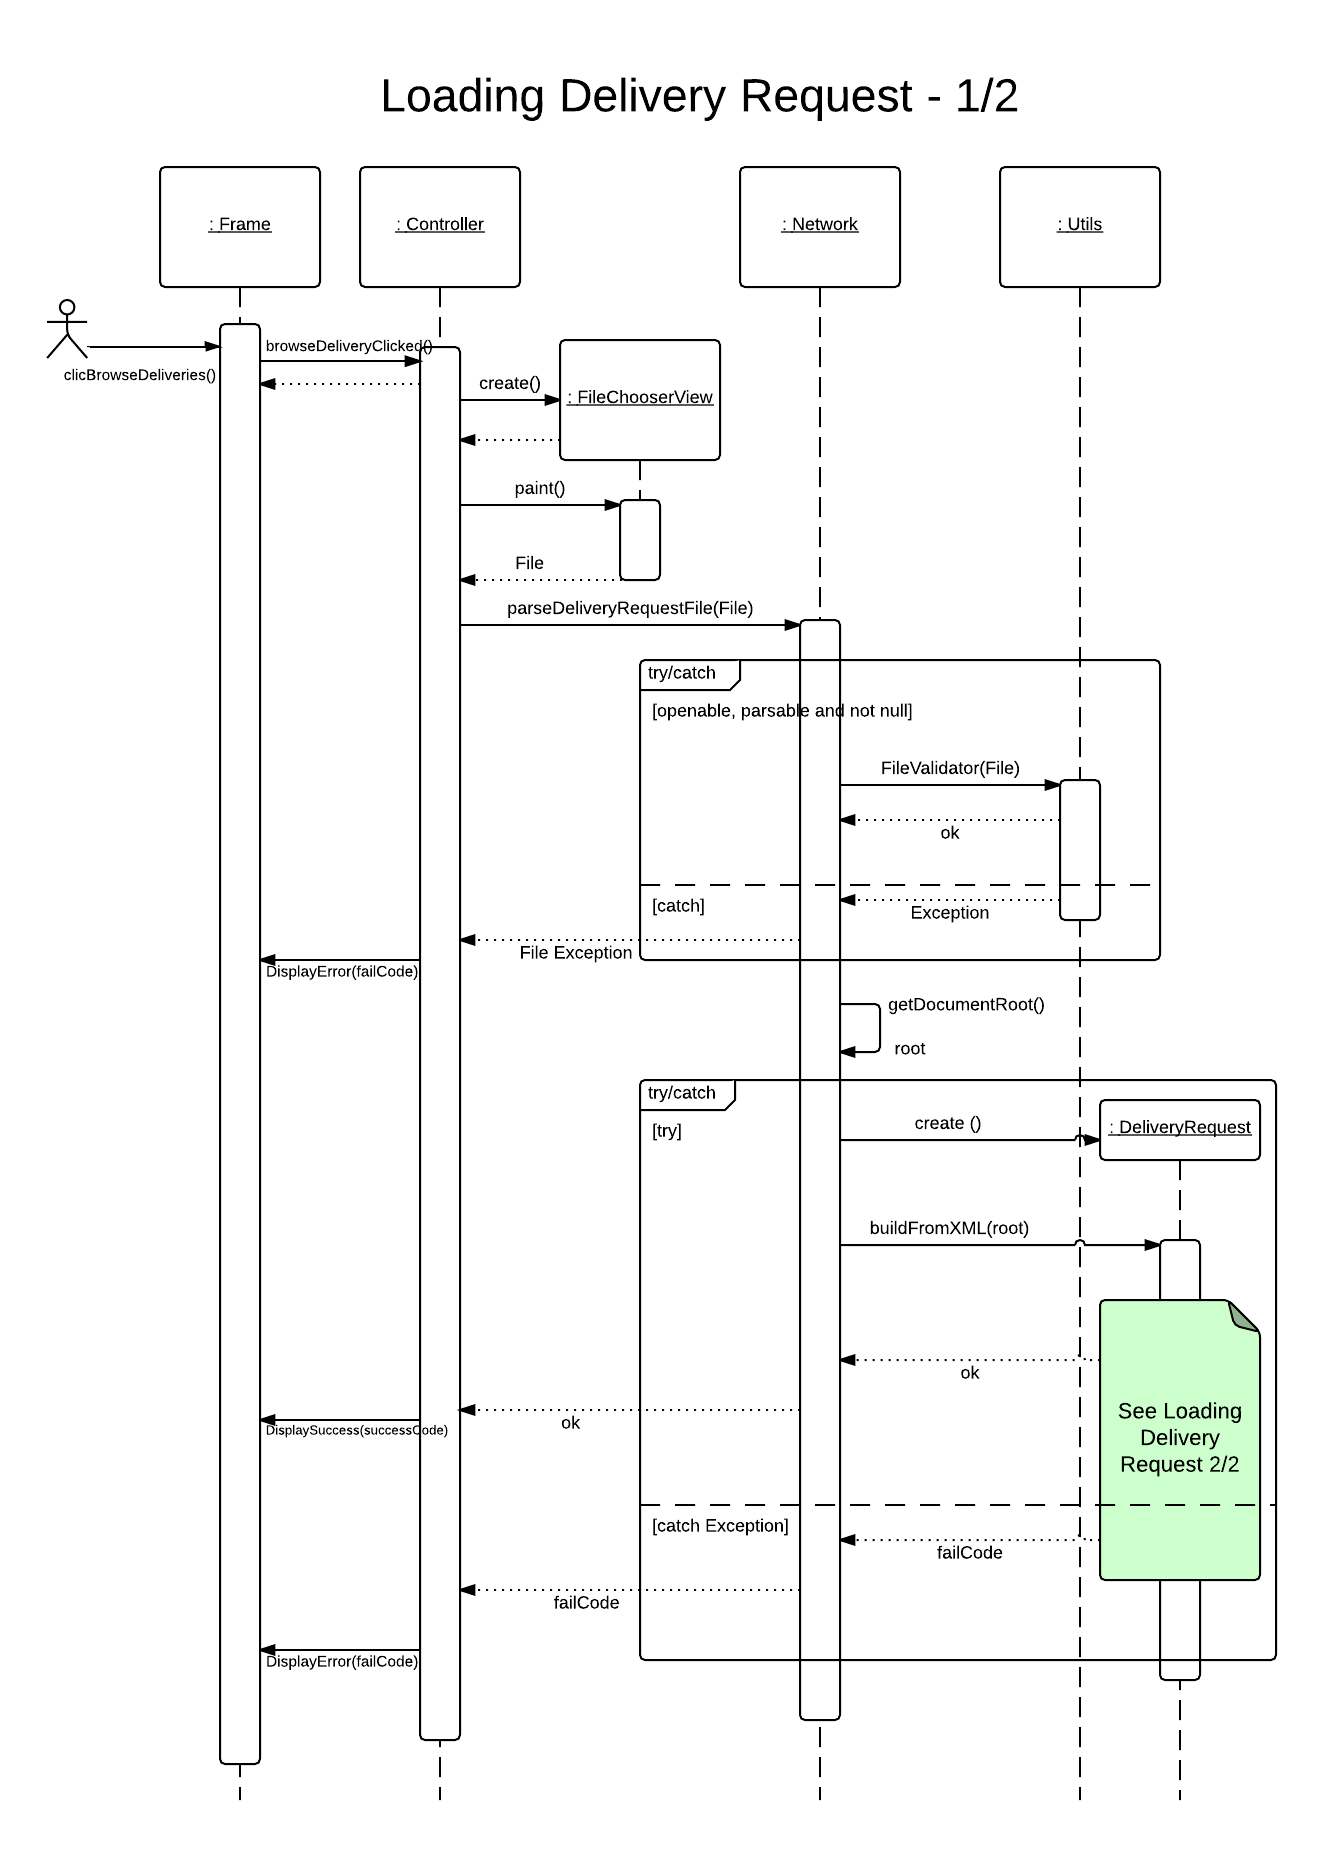
\includegraphics[width=\textwidth,height=\textheight,keepaspectratio]{Figures/chargement1}
		\rule{35em}{0.5pt}
	\caption[Chargement d'une demande de livraison - Partie 1]{Chargement d'une demande de livraison - Partie 1}
\end{figure}

\begin{figure}[H]
	\centering
		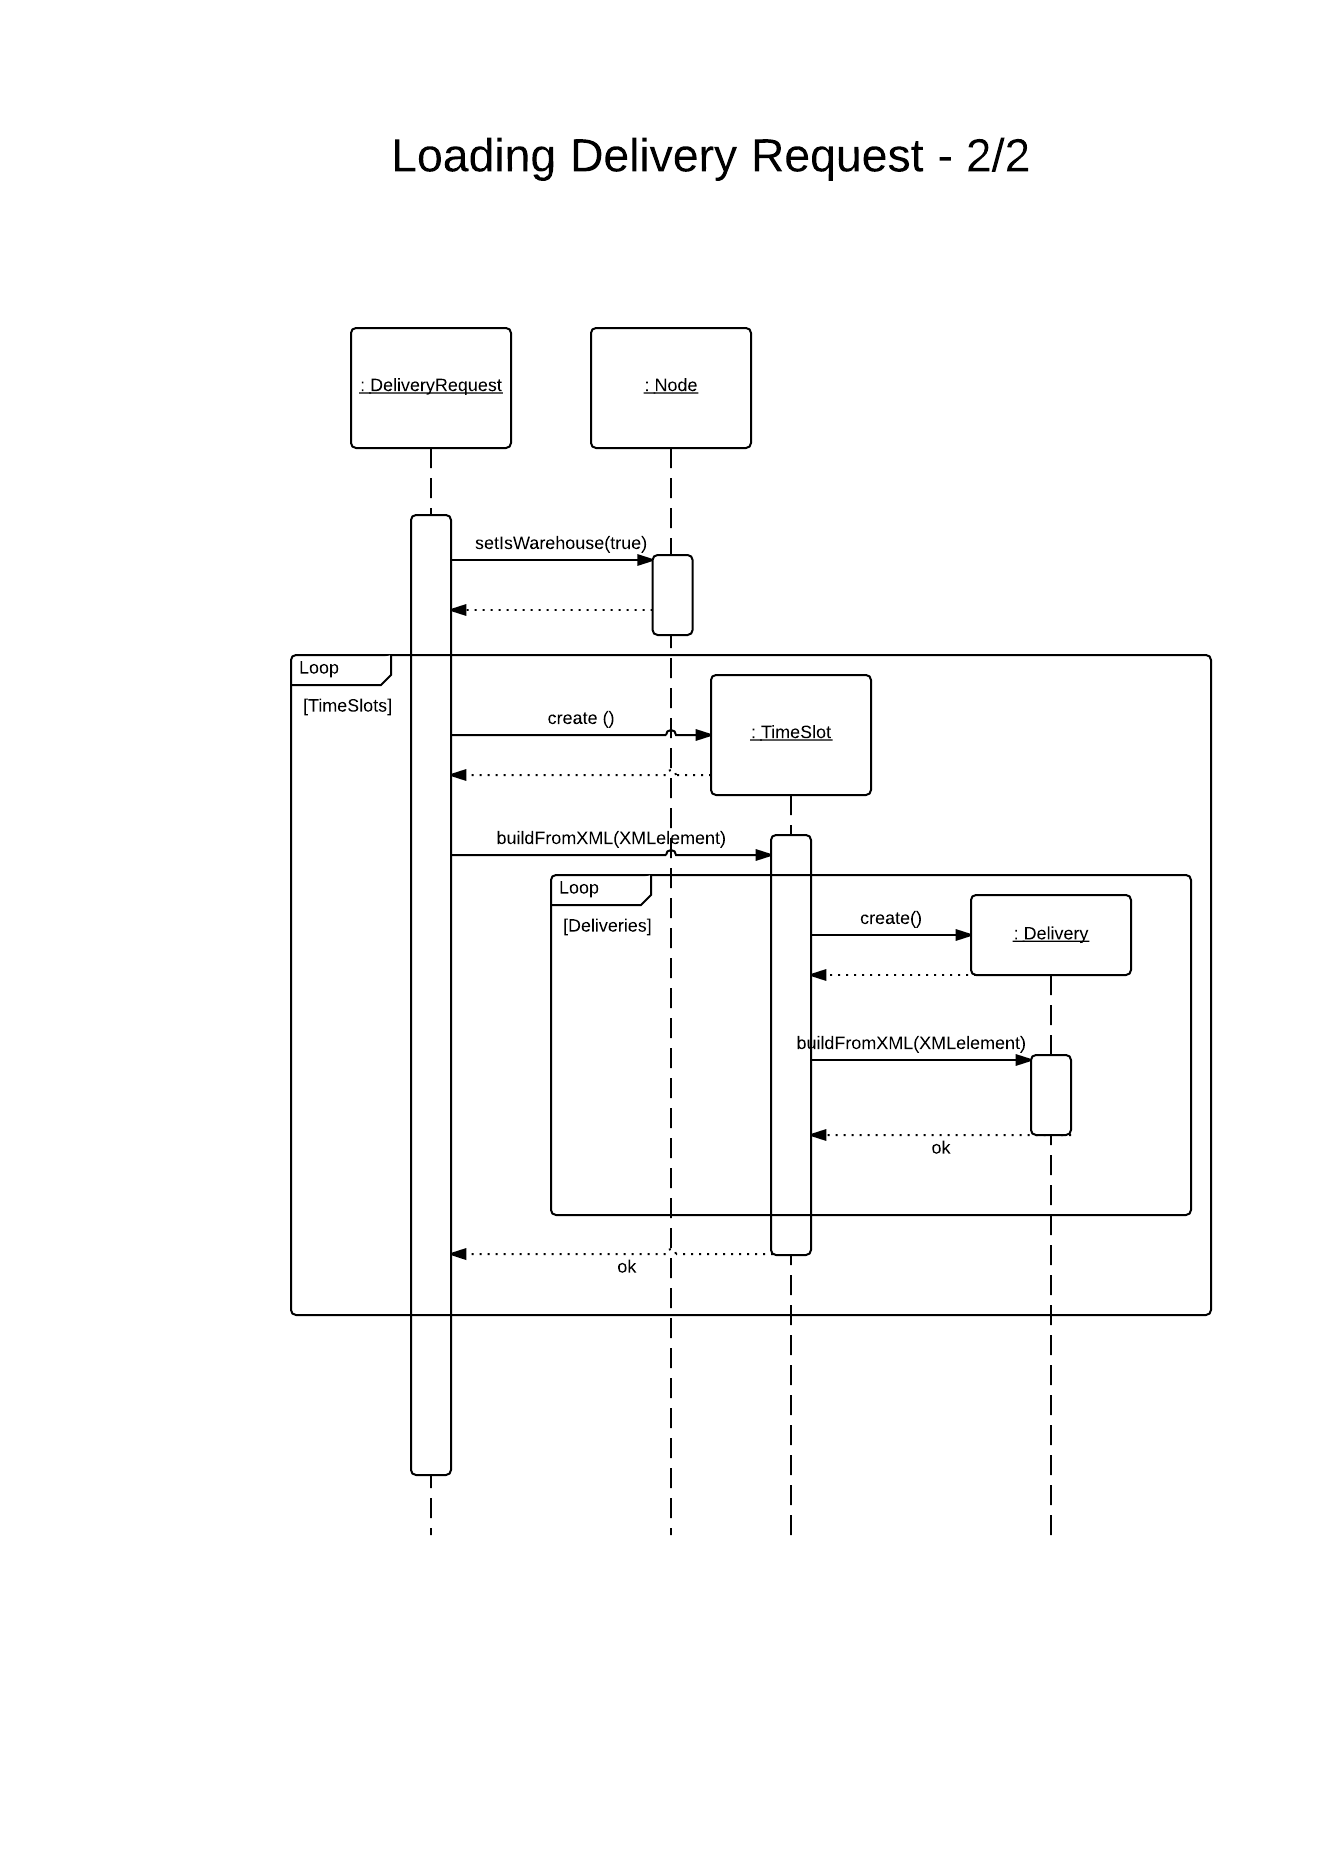
\includegraphics[width=\textwidth,height=\textheight,keepaspectratio]{Figures/chargement2}
		\rule{35em}{0.5pt}
	\caption[Chargement d'une demande de livraison - Partie 2]{Chargement d'une demande de livraison - Partie 2}
\end{figure}

\subsection{Calcul d'une tournée}
\begin{figure}[H]
	\centering
		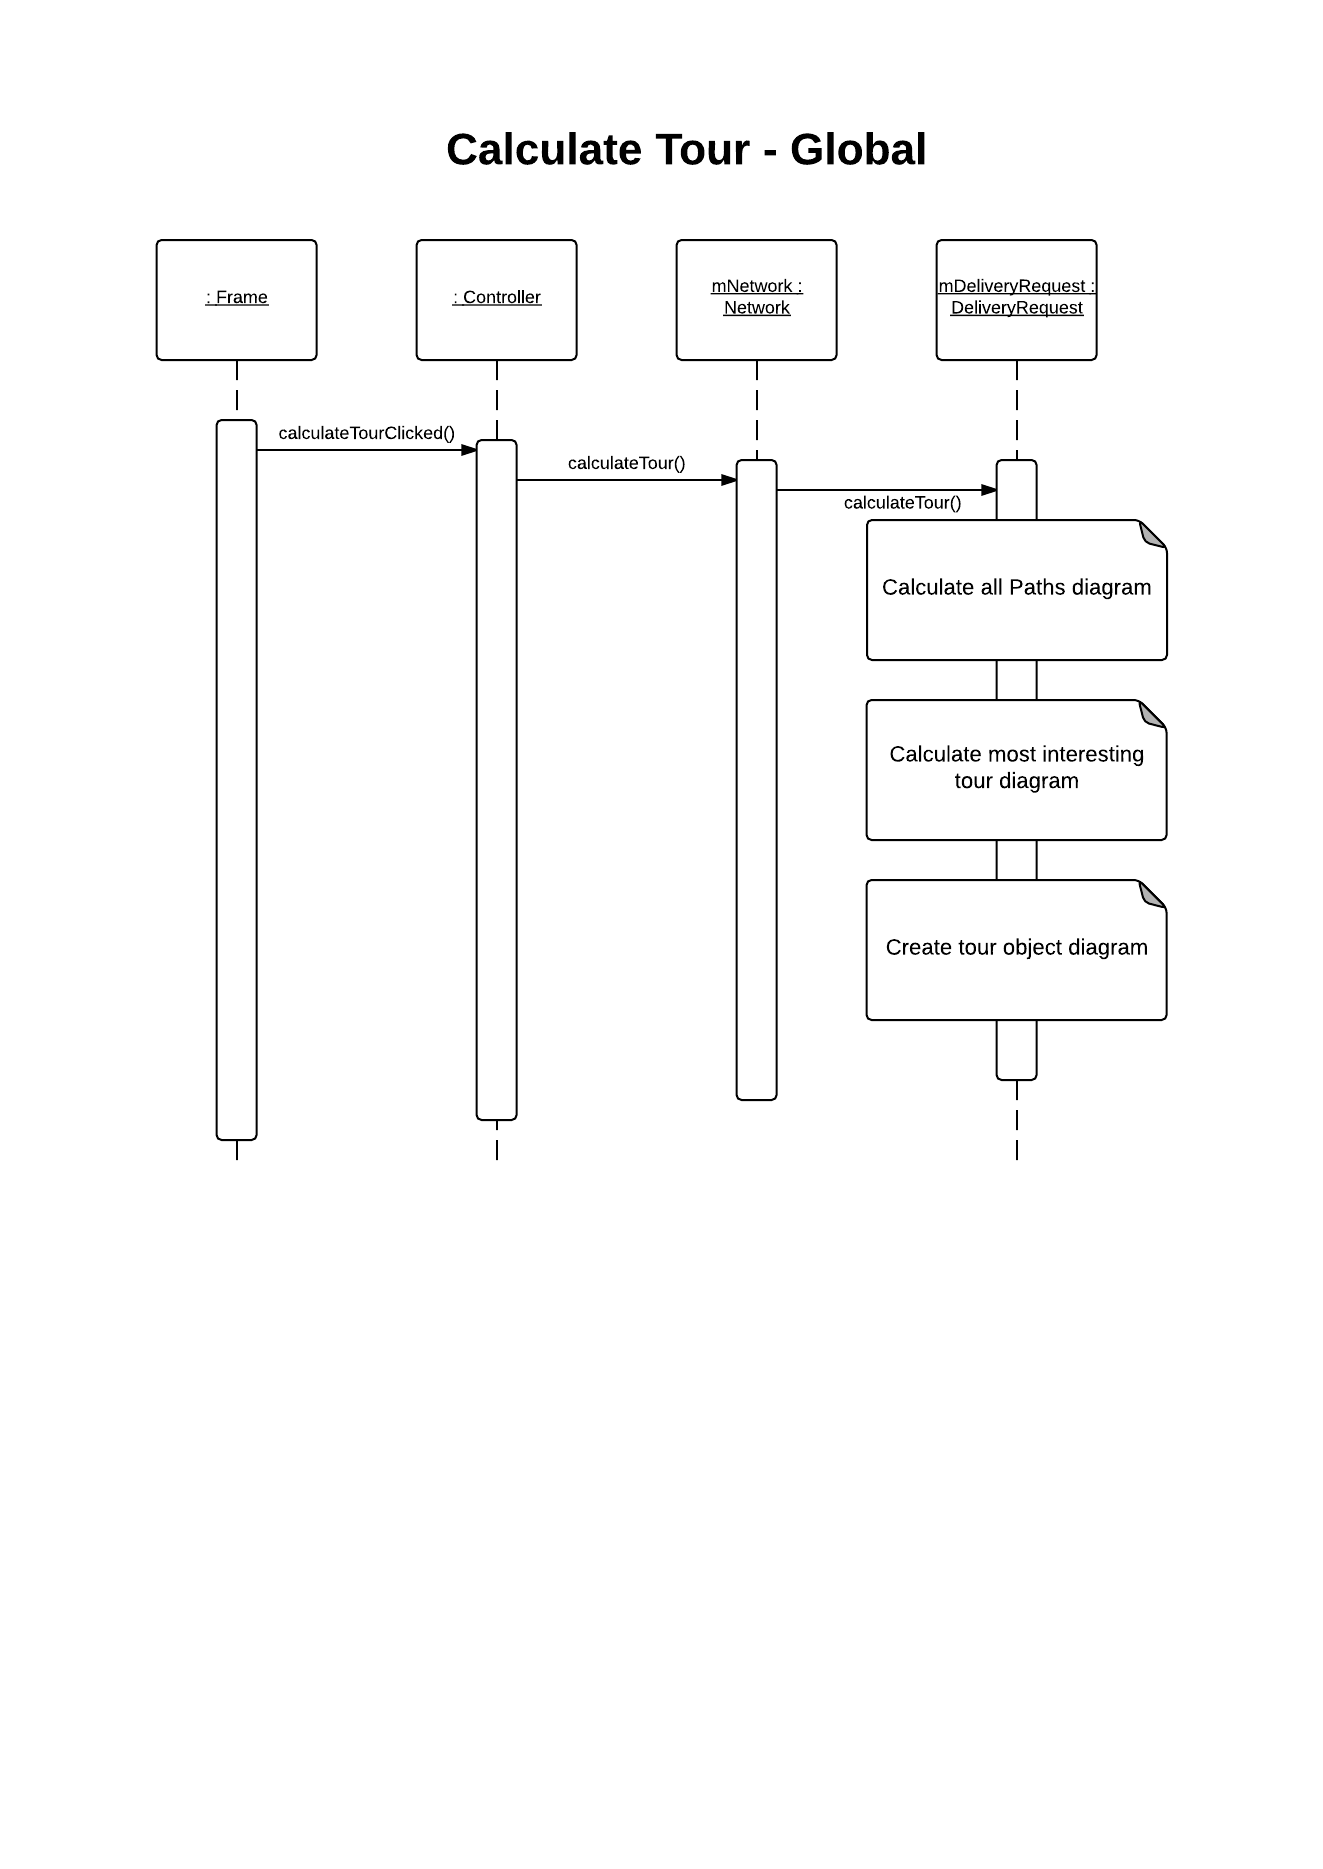
\includegraphics[width=\textwidth,height=\textheight,keepaspectratio]{Figures/calcul_tournee1}
		\rule{35em}{0.5pt}
	\caption[Calcul d'une tournée-général]{Calcul d'une tournée-général}
\end{figure}

\begin{figure}[H]
	\centering
		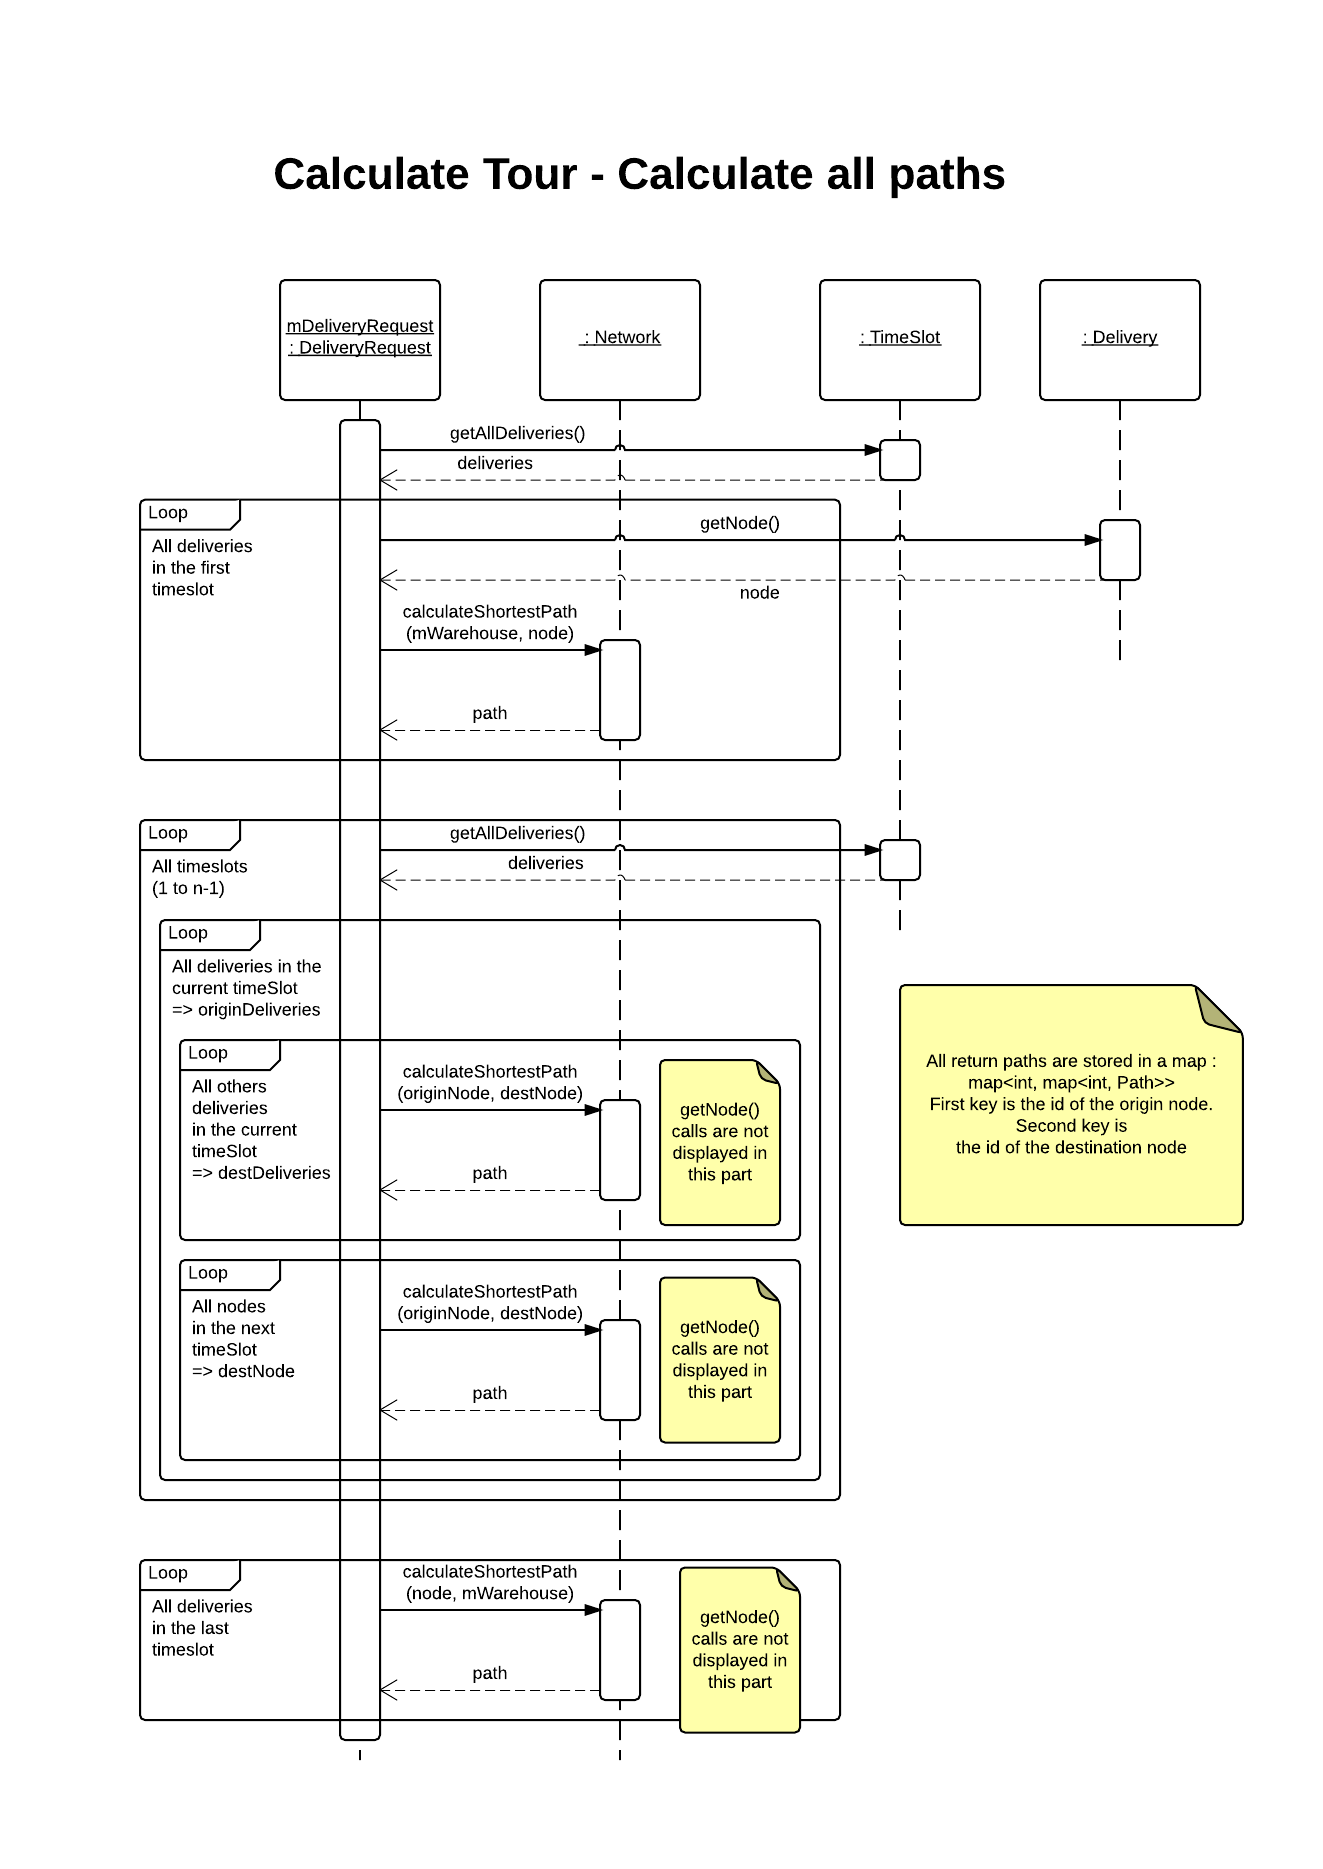
\includegraphics[width=\textwidth,height=\textheight,keepaspectratio]{Figures/calcul_tournee2}
		\rule{35em}{0.5pt}
	\caption[Calcul des plus courts chemins]{Calcul des plus courts chemins}
\end{figure}

\begin{figure}[H]
	\centering
		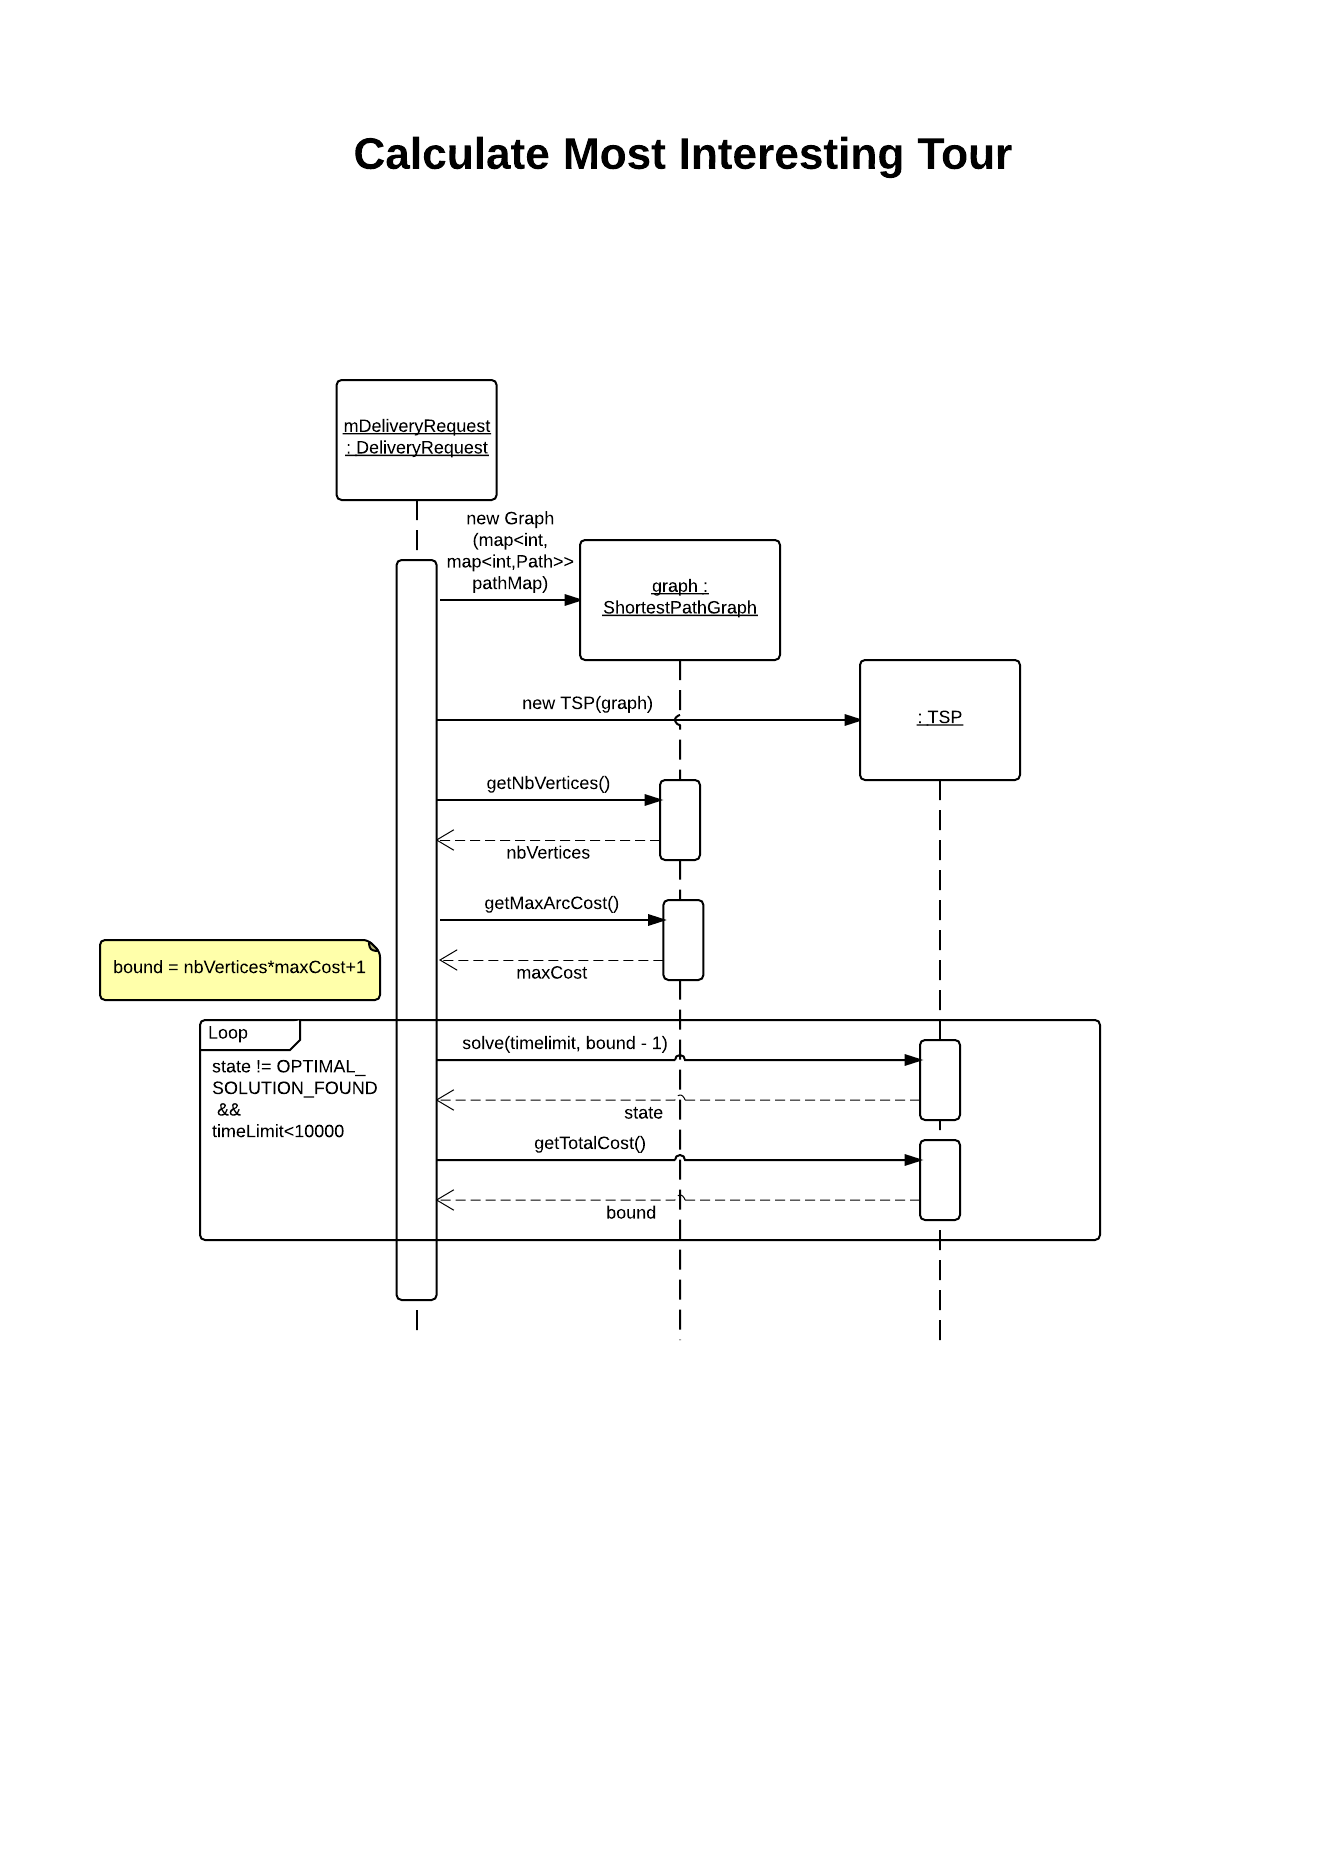
\includegraphics[width=\textwidth,height=\textheight,keepaspectratio]{Figures/calcul_tournee3}
		\rule{35em}{0.5pt}
	\caption[Calcul de la tournée la plus intéressante]{Calcul de la tournée la plus intéressante}
\end{figure}

\begin{figure}[H]
	\centering
		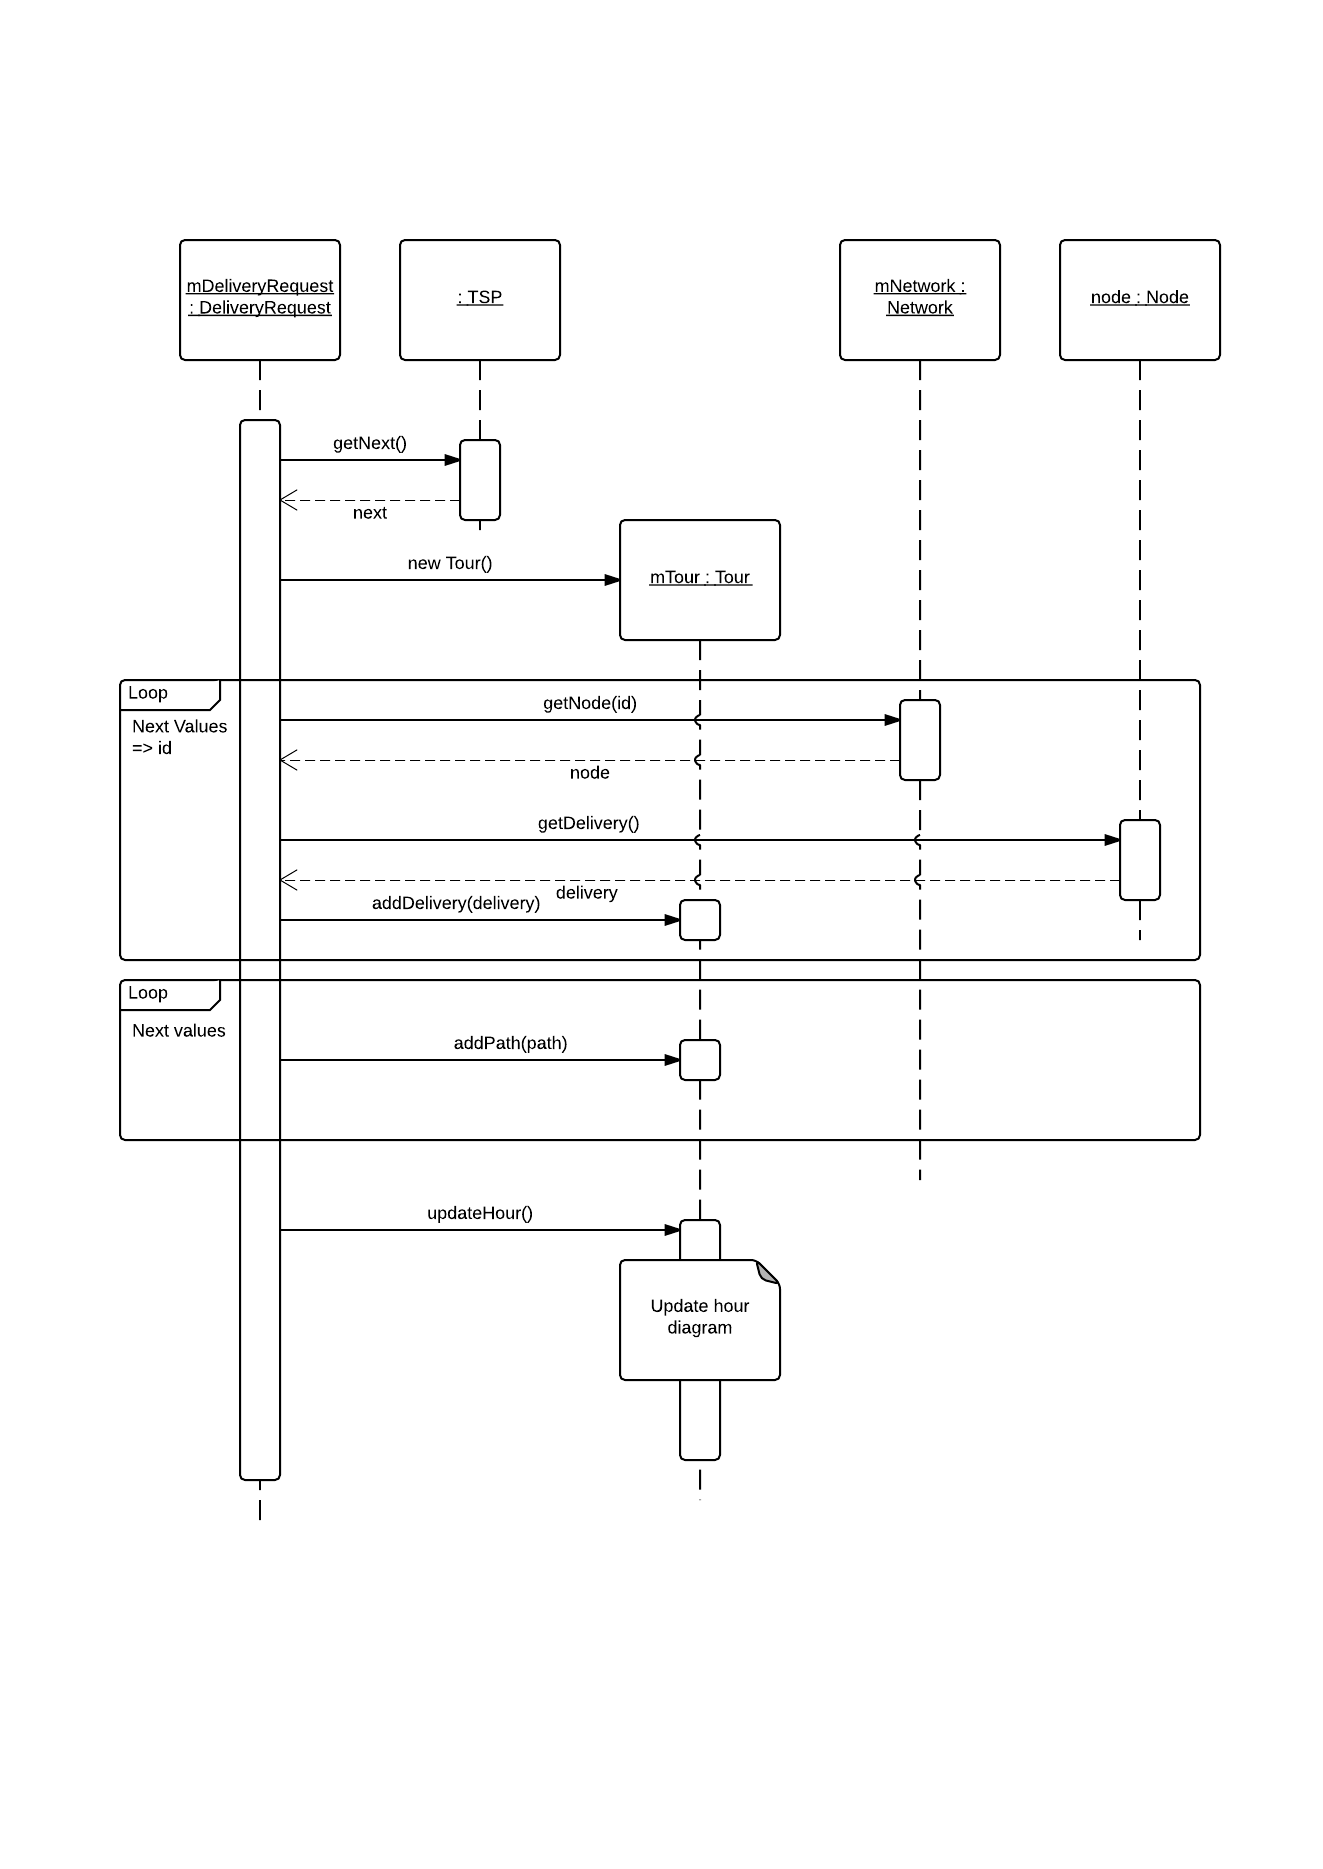
\includegraphics[width=\textwidth,height=\textheight,keepaspectratio]{Figures/calcul_tournee4}
		\rule{35em}{0.5pt}
	\caption[Construction de l'itinéraire]{Construction de l'itinéraire}
\end{figure}

\begin{figure}[H]
	\centering
		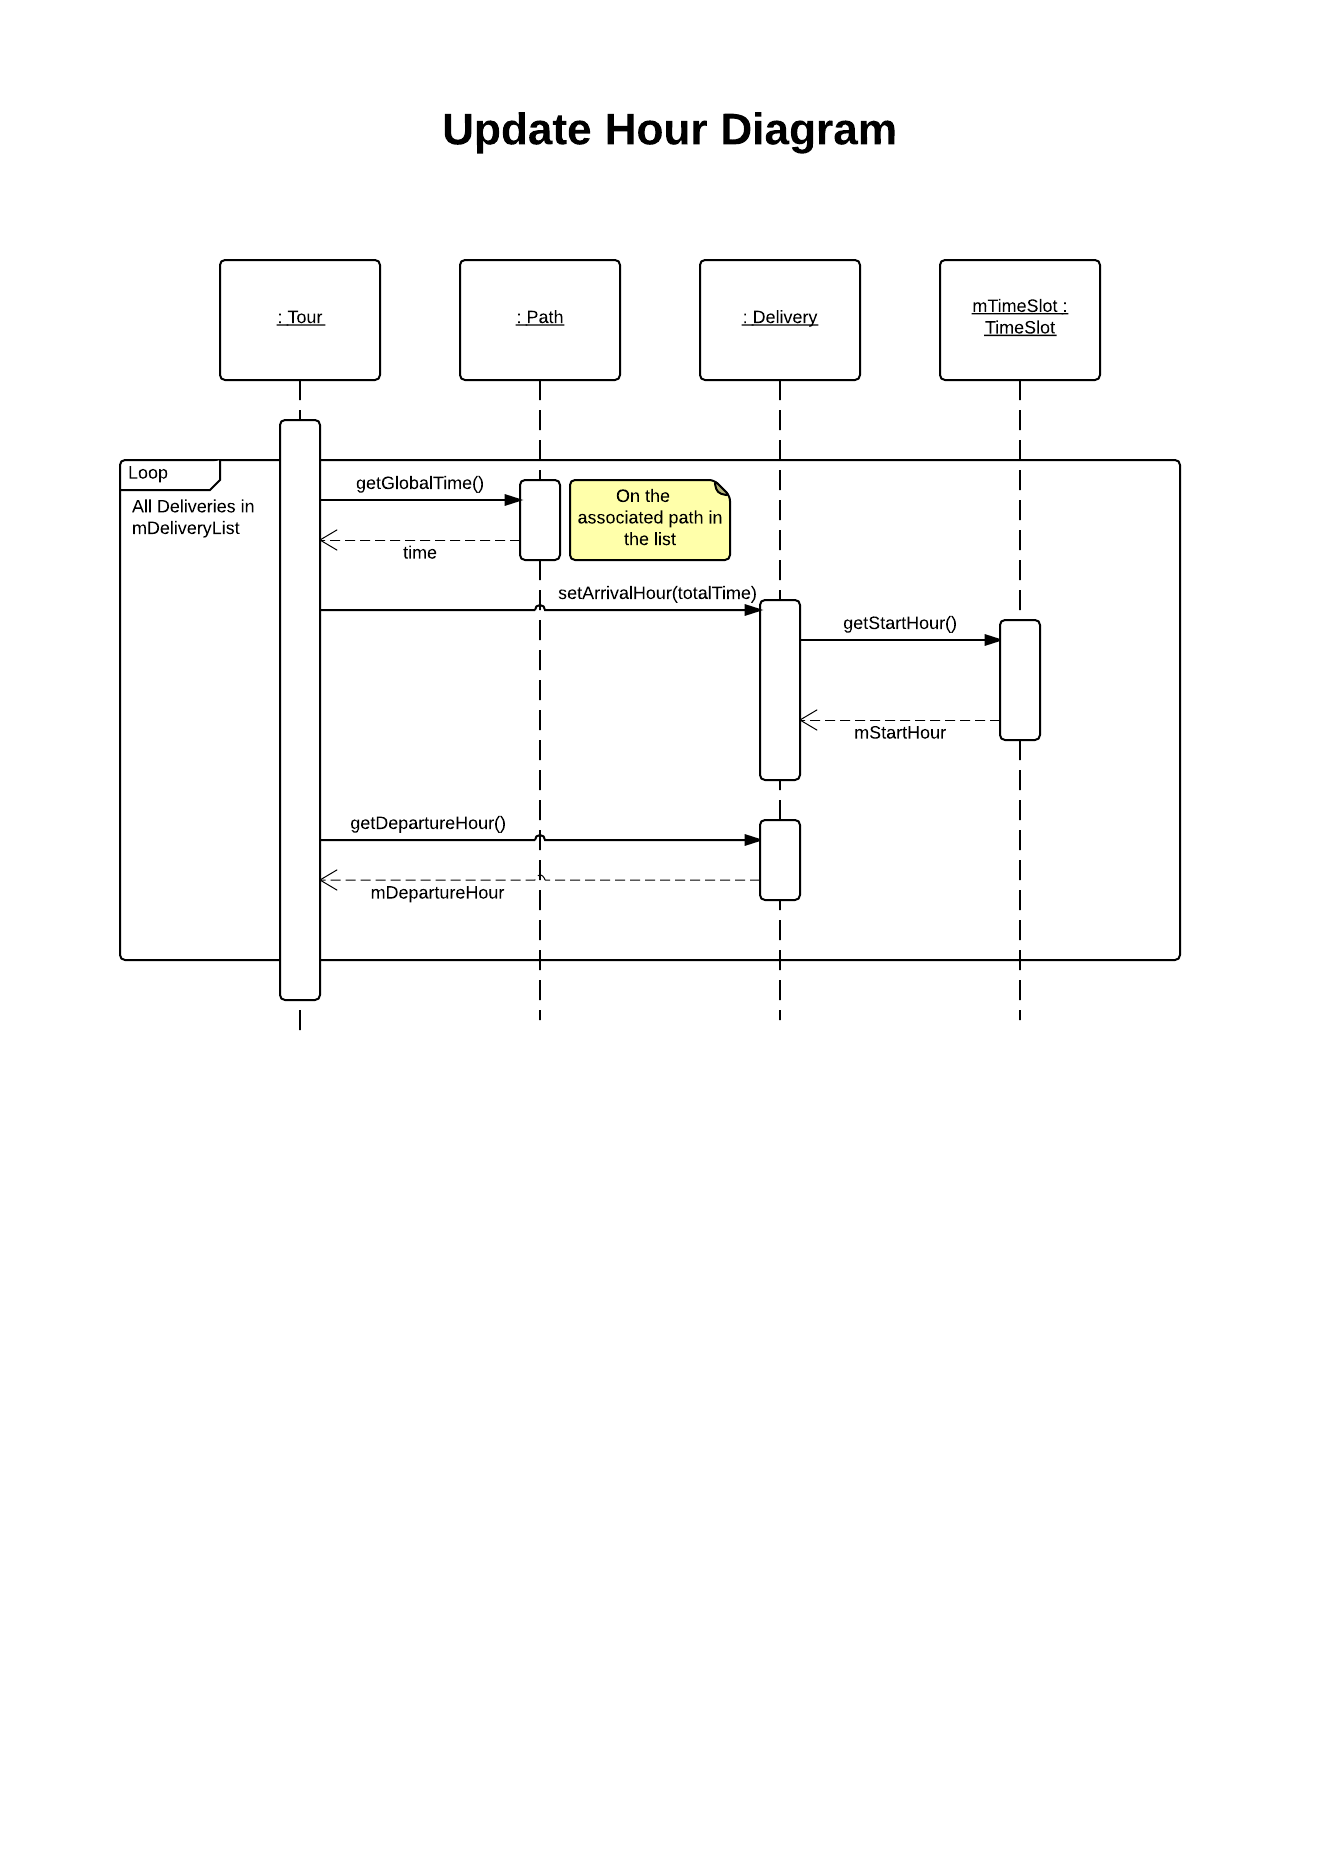
\includegraphics[width=\textwidth,height=\textheight,keepaspectratio, angle=90]{Figures/heure}
		\rule{35em}{0.5pt}
	\caption[Mise à jour de l'heure de livraison]{Mise à jour de l'heure de livraison}
\end{figure}


\subsection{Insertion d'un point de livraison dans une demande de livraison}

\begin{figure}[H]
	\centering
		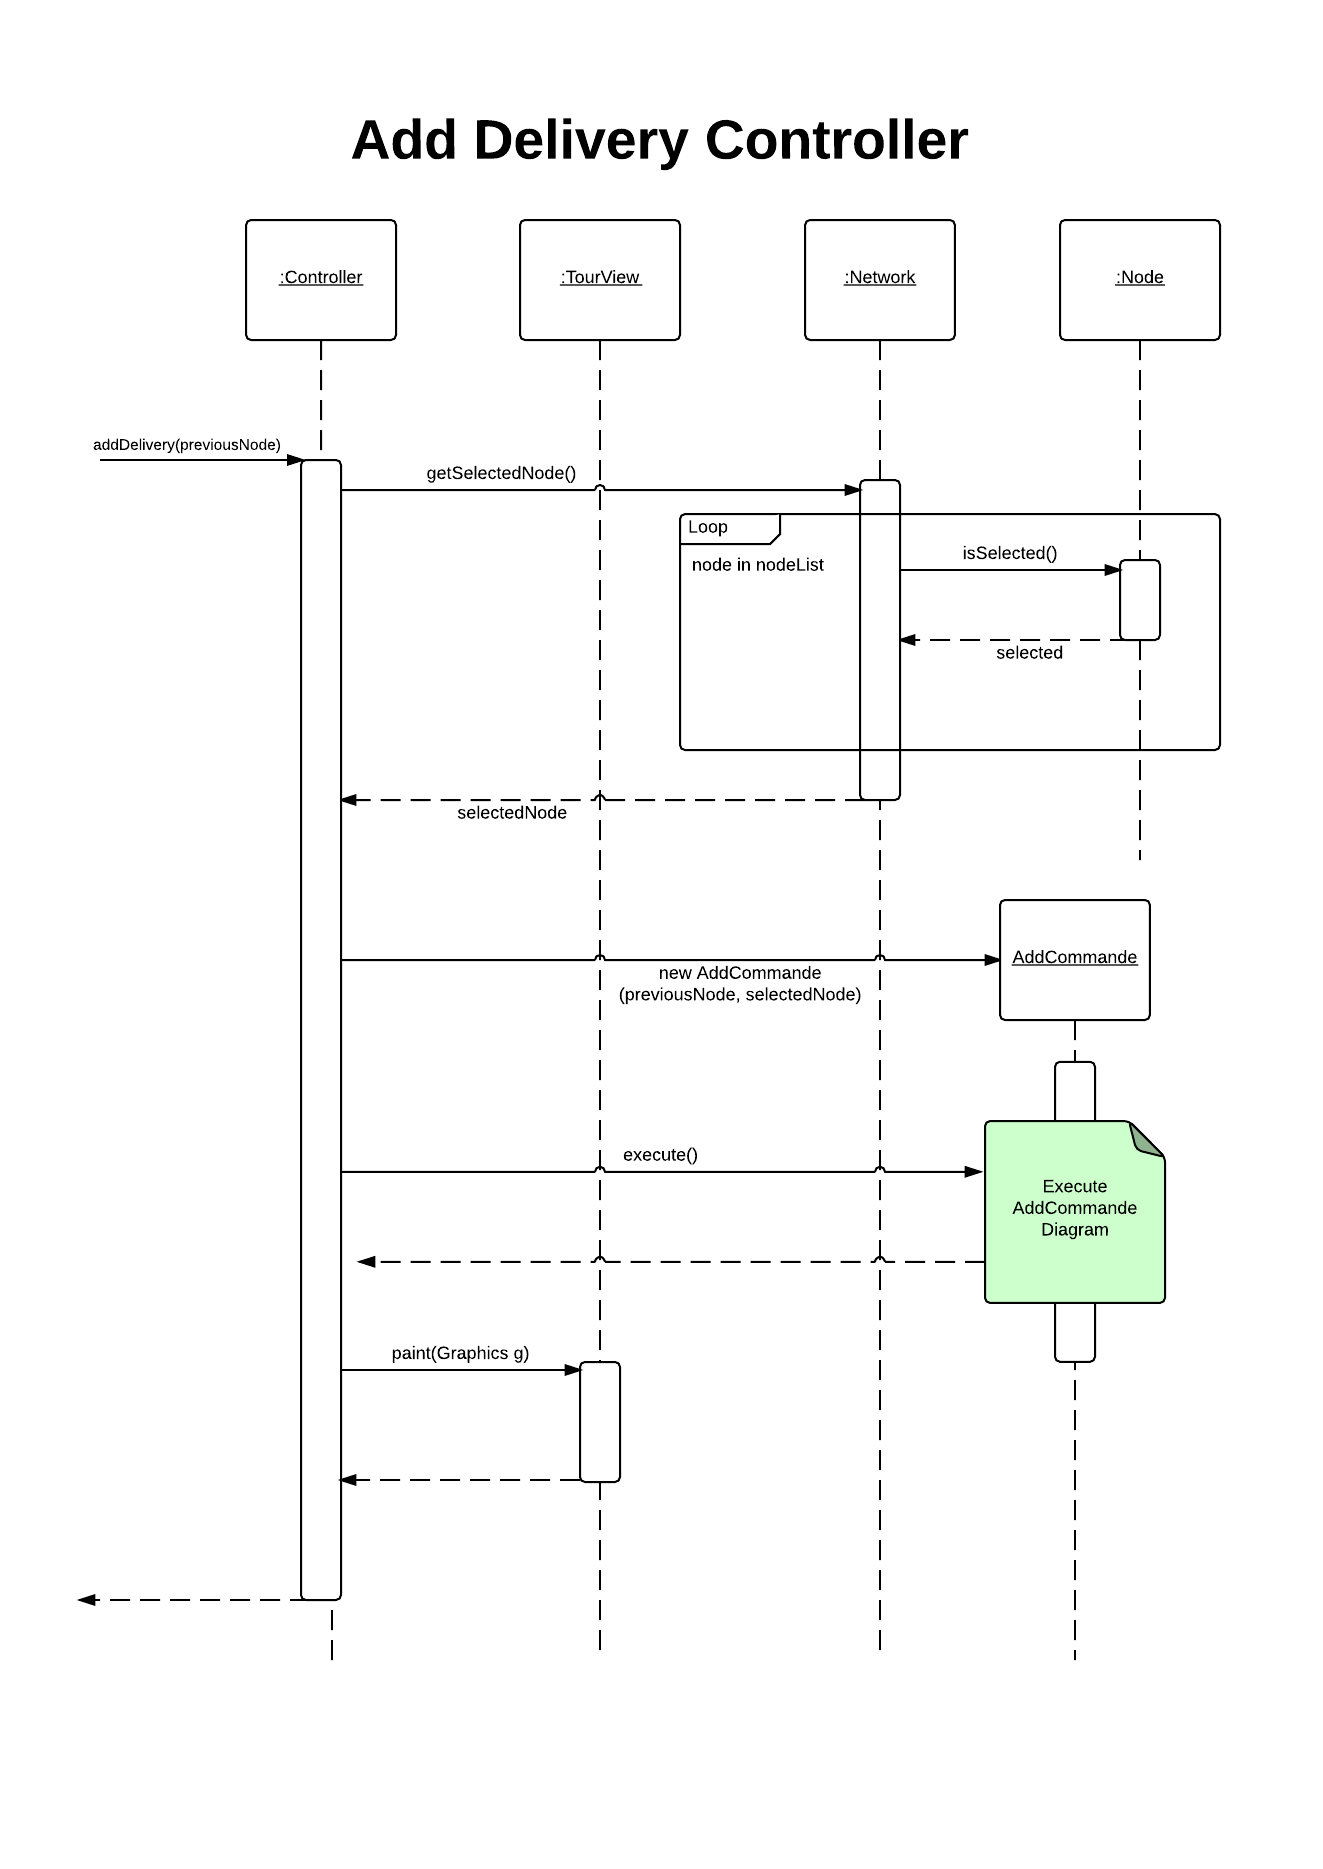
\includegraphics[width=\textwidth,height=\textheight,keepaspectratio]{Figures/ajout_livraison1}
		\rule{35em}{0.5pt}
	\caption[Ajout d'une livraison - diagramme général]{Ajout d'une livraison - diagramme général}
\end{figure}
\clearpage
\begin{figure}[H]
	\centering
		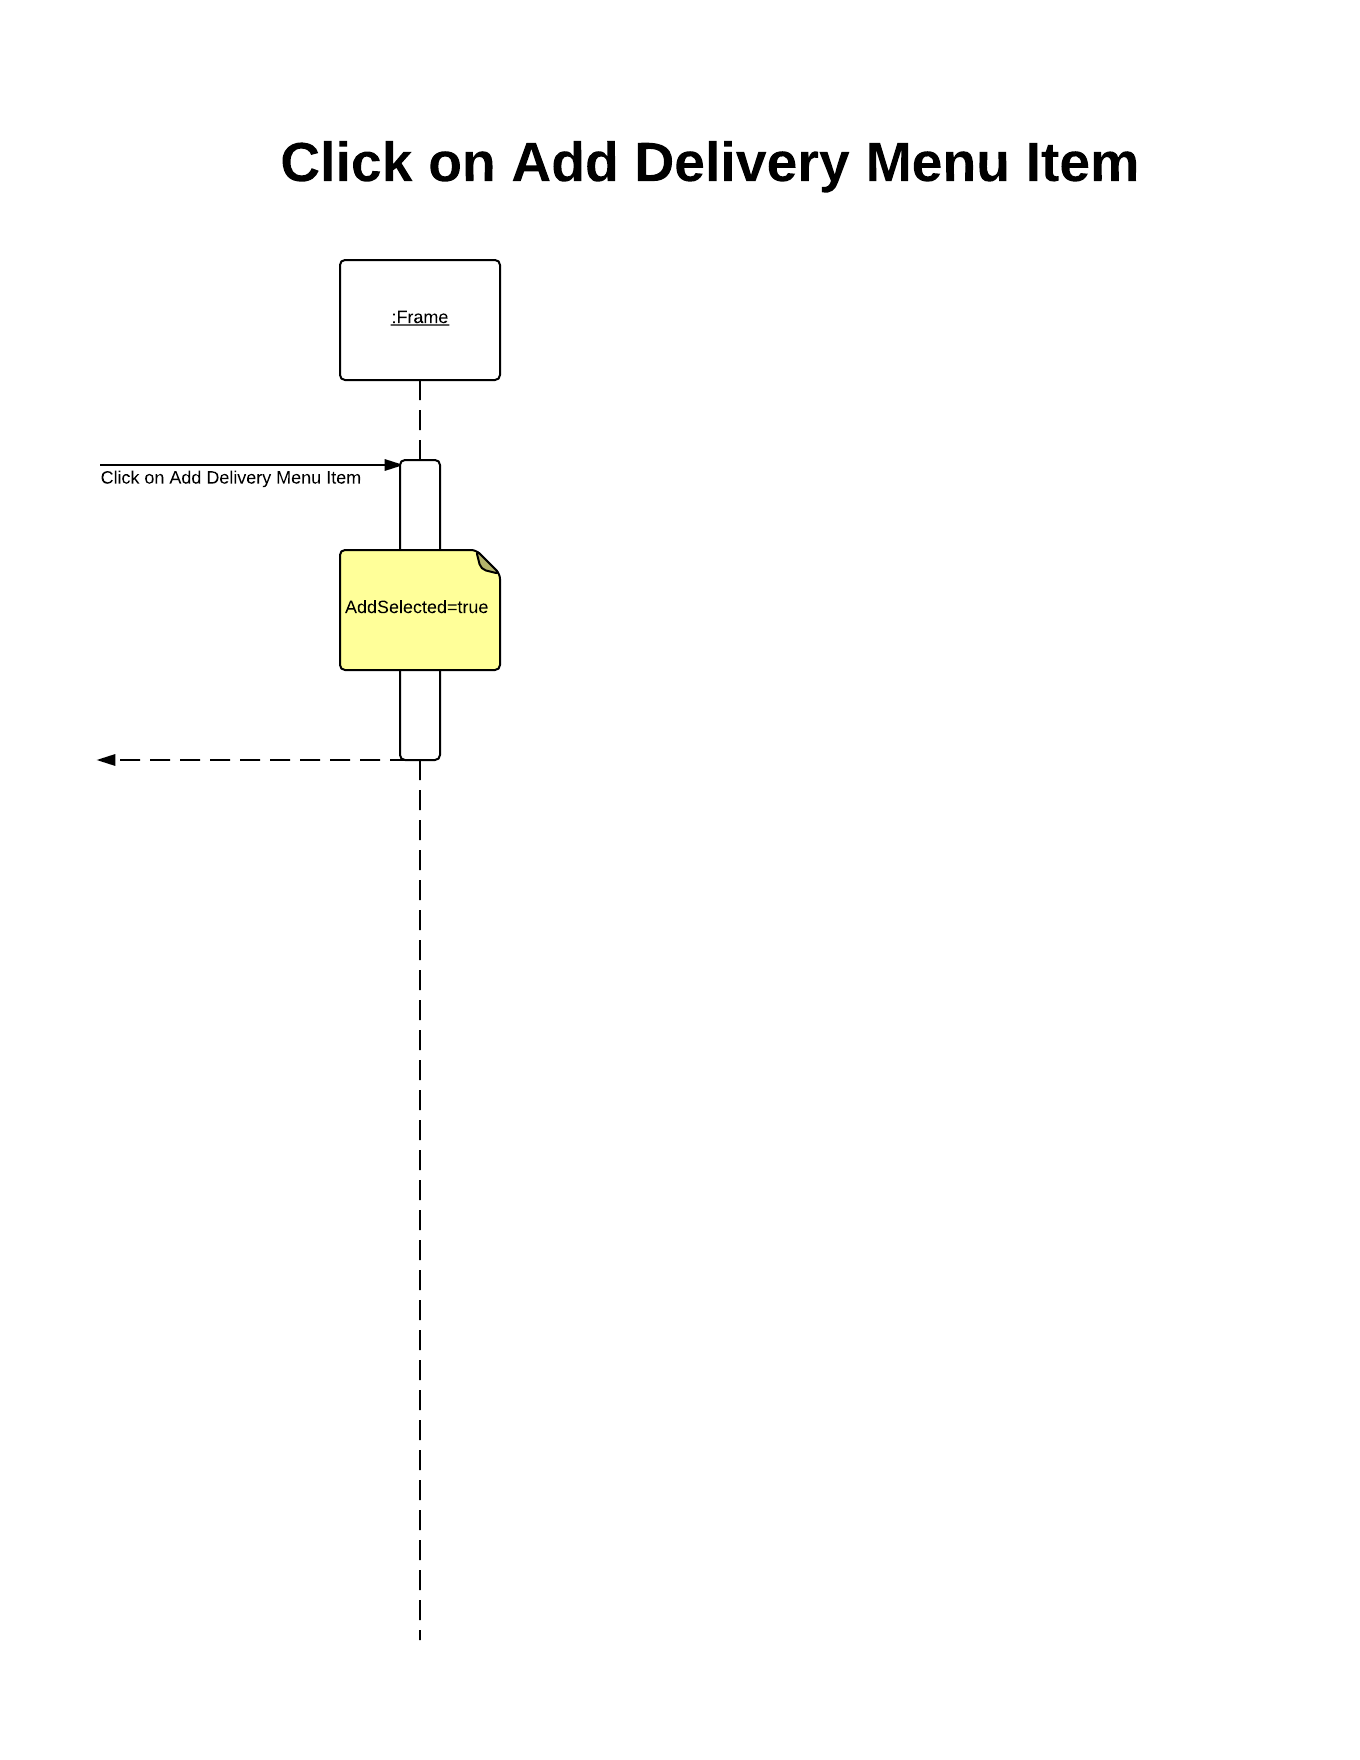
\includegraphics[width=\textwidth,height=\textheight,keepaspectratio]{Figures/ajout_livraison2}
		\rule{35em}{0.5pt}
	\caption[Click sur le menu]{Click sur le menu}
\end{figure}

\clearpage
\begin{figure}[H]
	\centering
		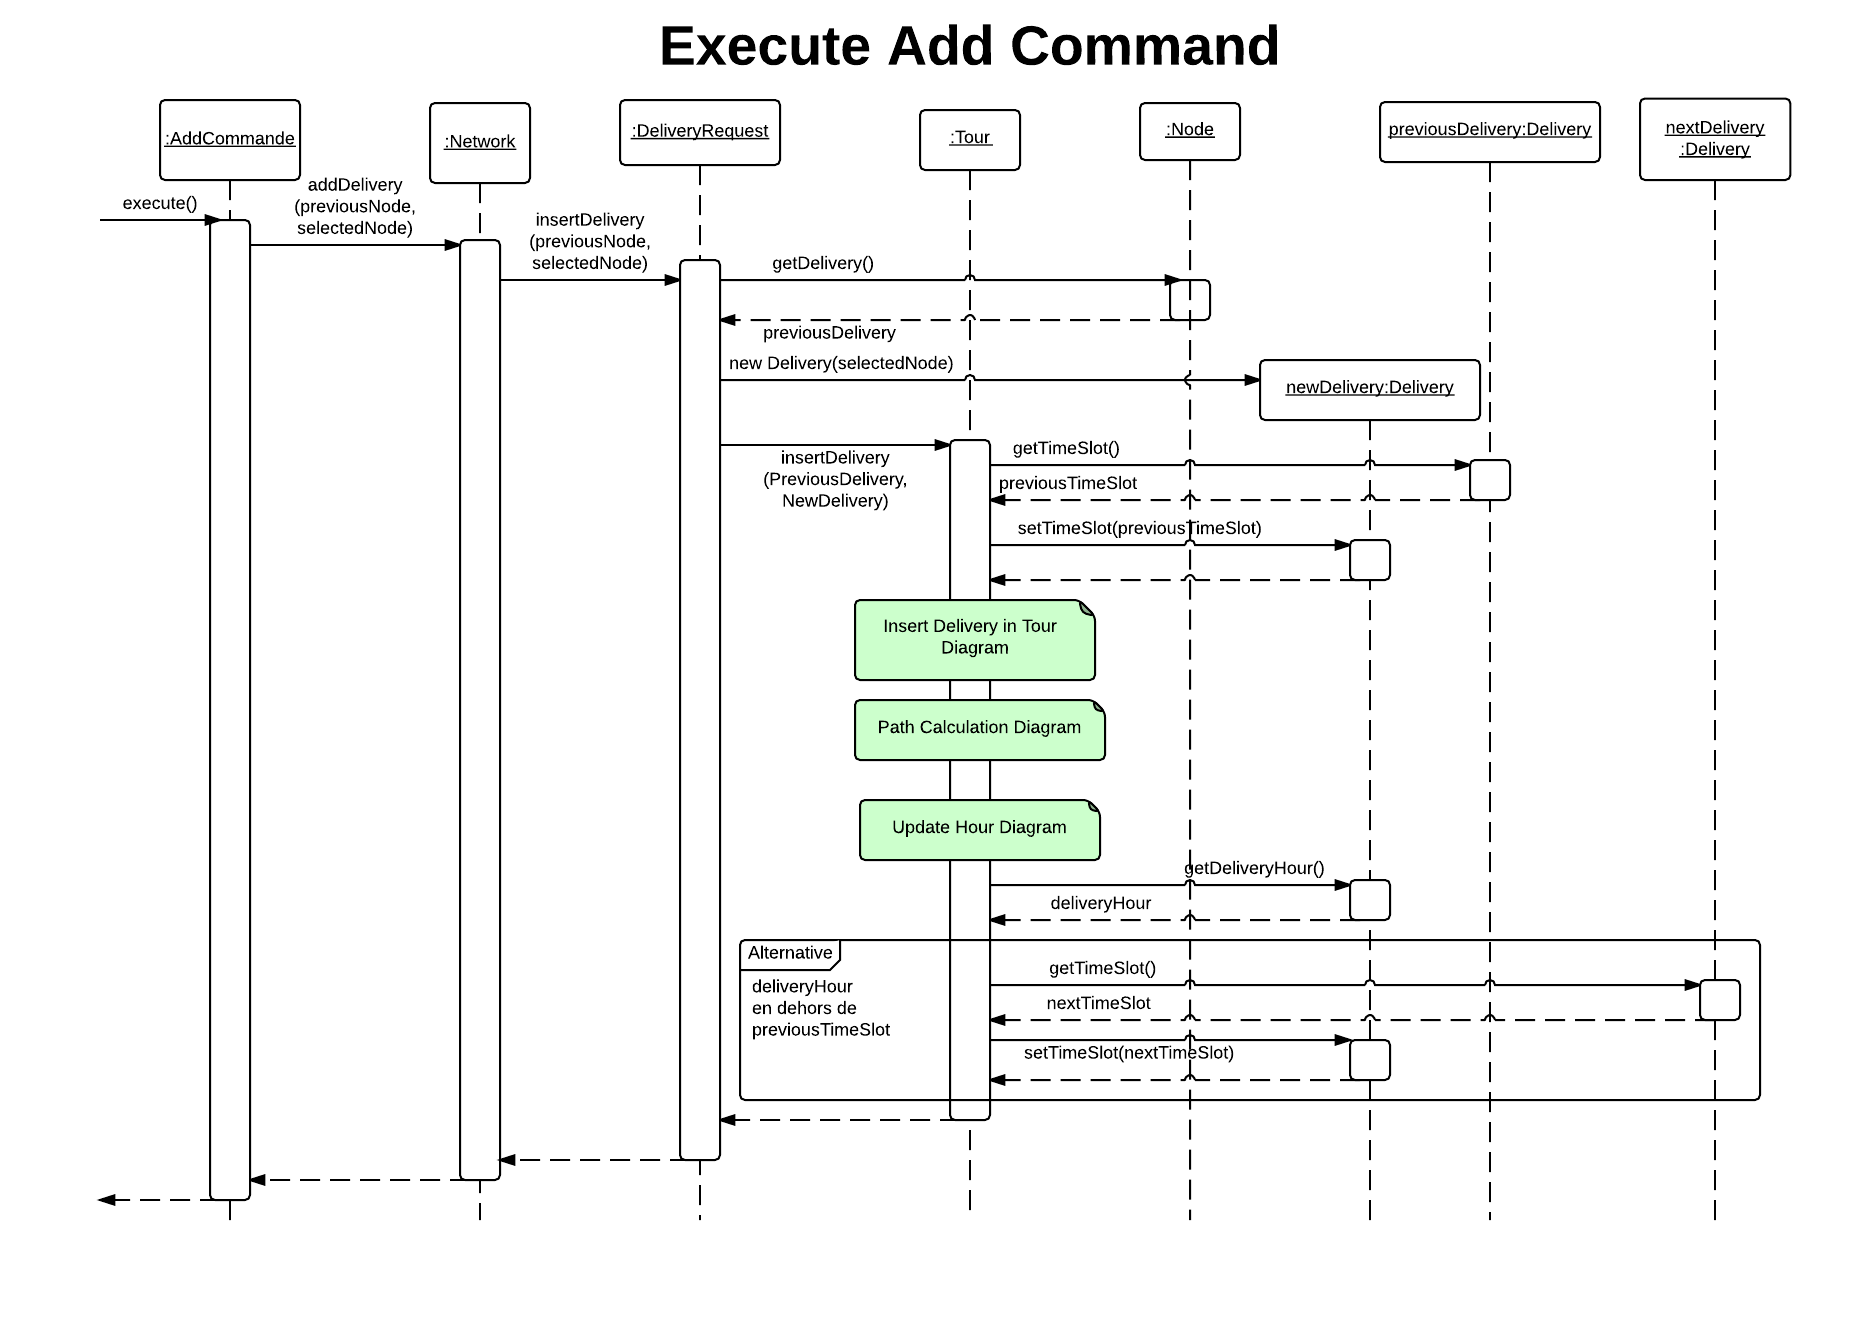
\includegraphics[width=\textwidth,height=\textheight,keepaspectratio, angle=90]{Figures/ajout_livraison3}
		\rule{35em}{0.5pt}
	\caption[Exécution de la commande Add]{Exécution de la commande Add }
\end{figure}

\clearpage
\begin{figure}[H]
	\centering
		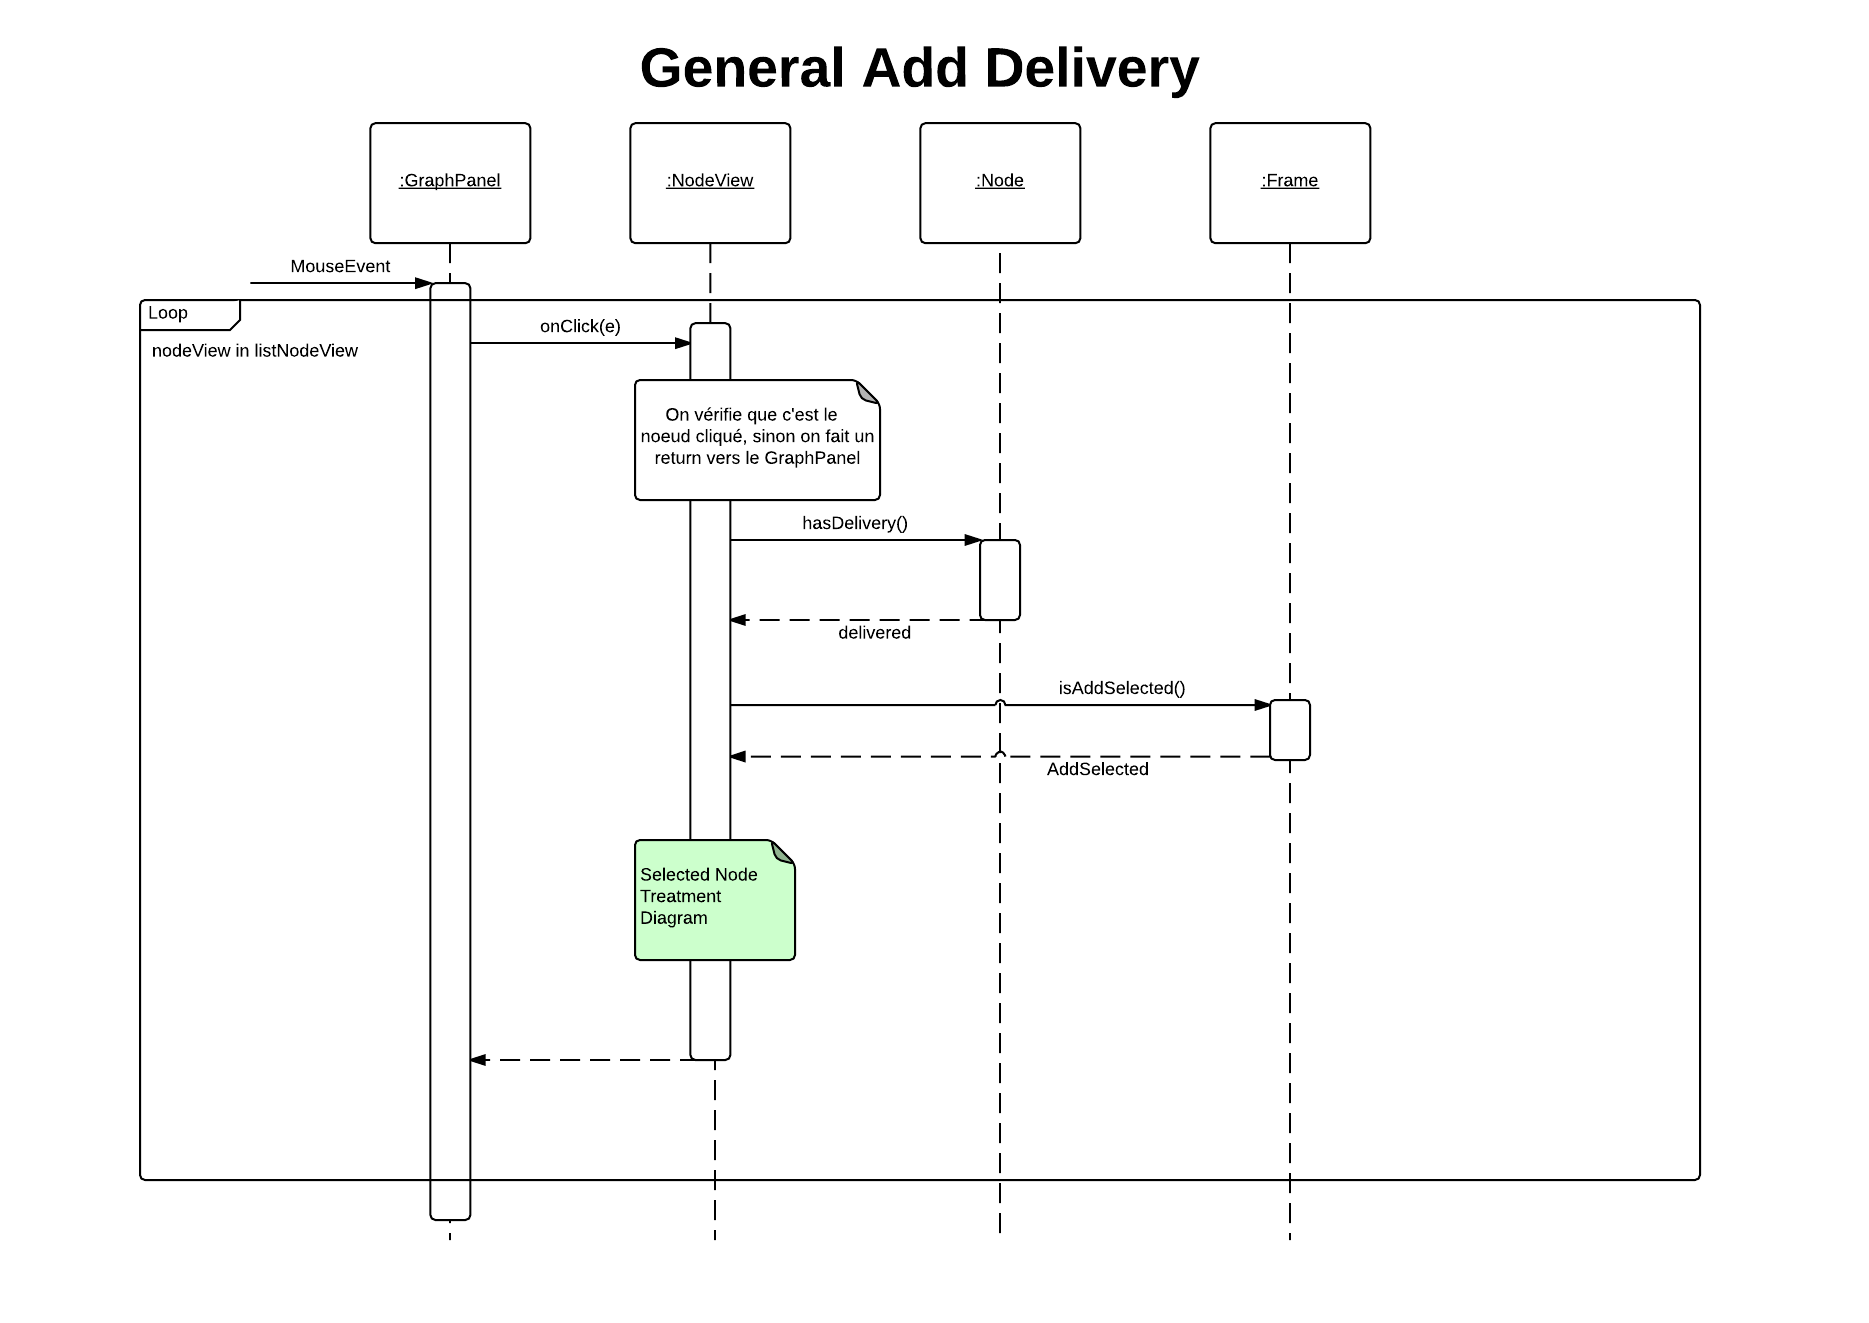
\includegraphics[width=\textwidth,height=\textheight,keepaspectratio, angle=90]{Figures/ajout_livraison4}
		\rule{35em}{0.5pt}
	\caption[Ajout d'une livraison]{Ajout d'une livraison}
\end{figure}

\begin{figure}[H]
	\centering
		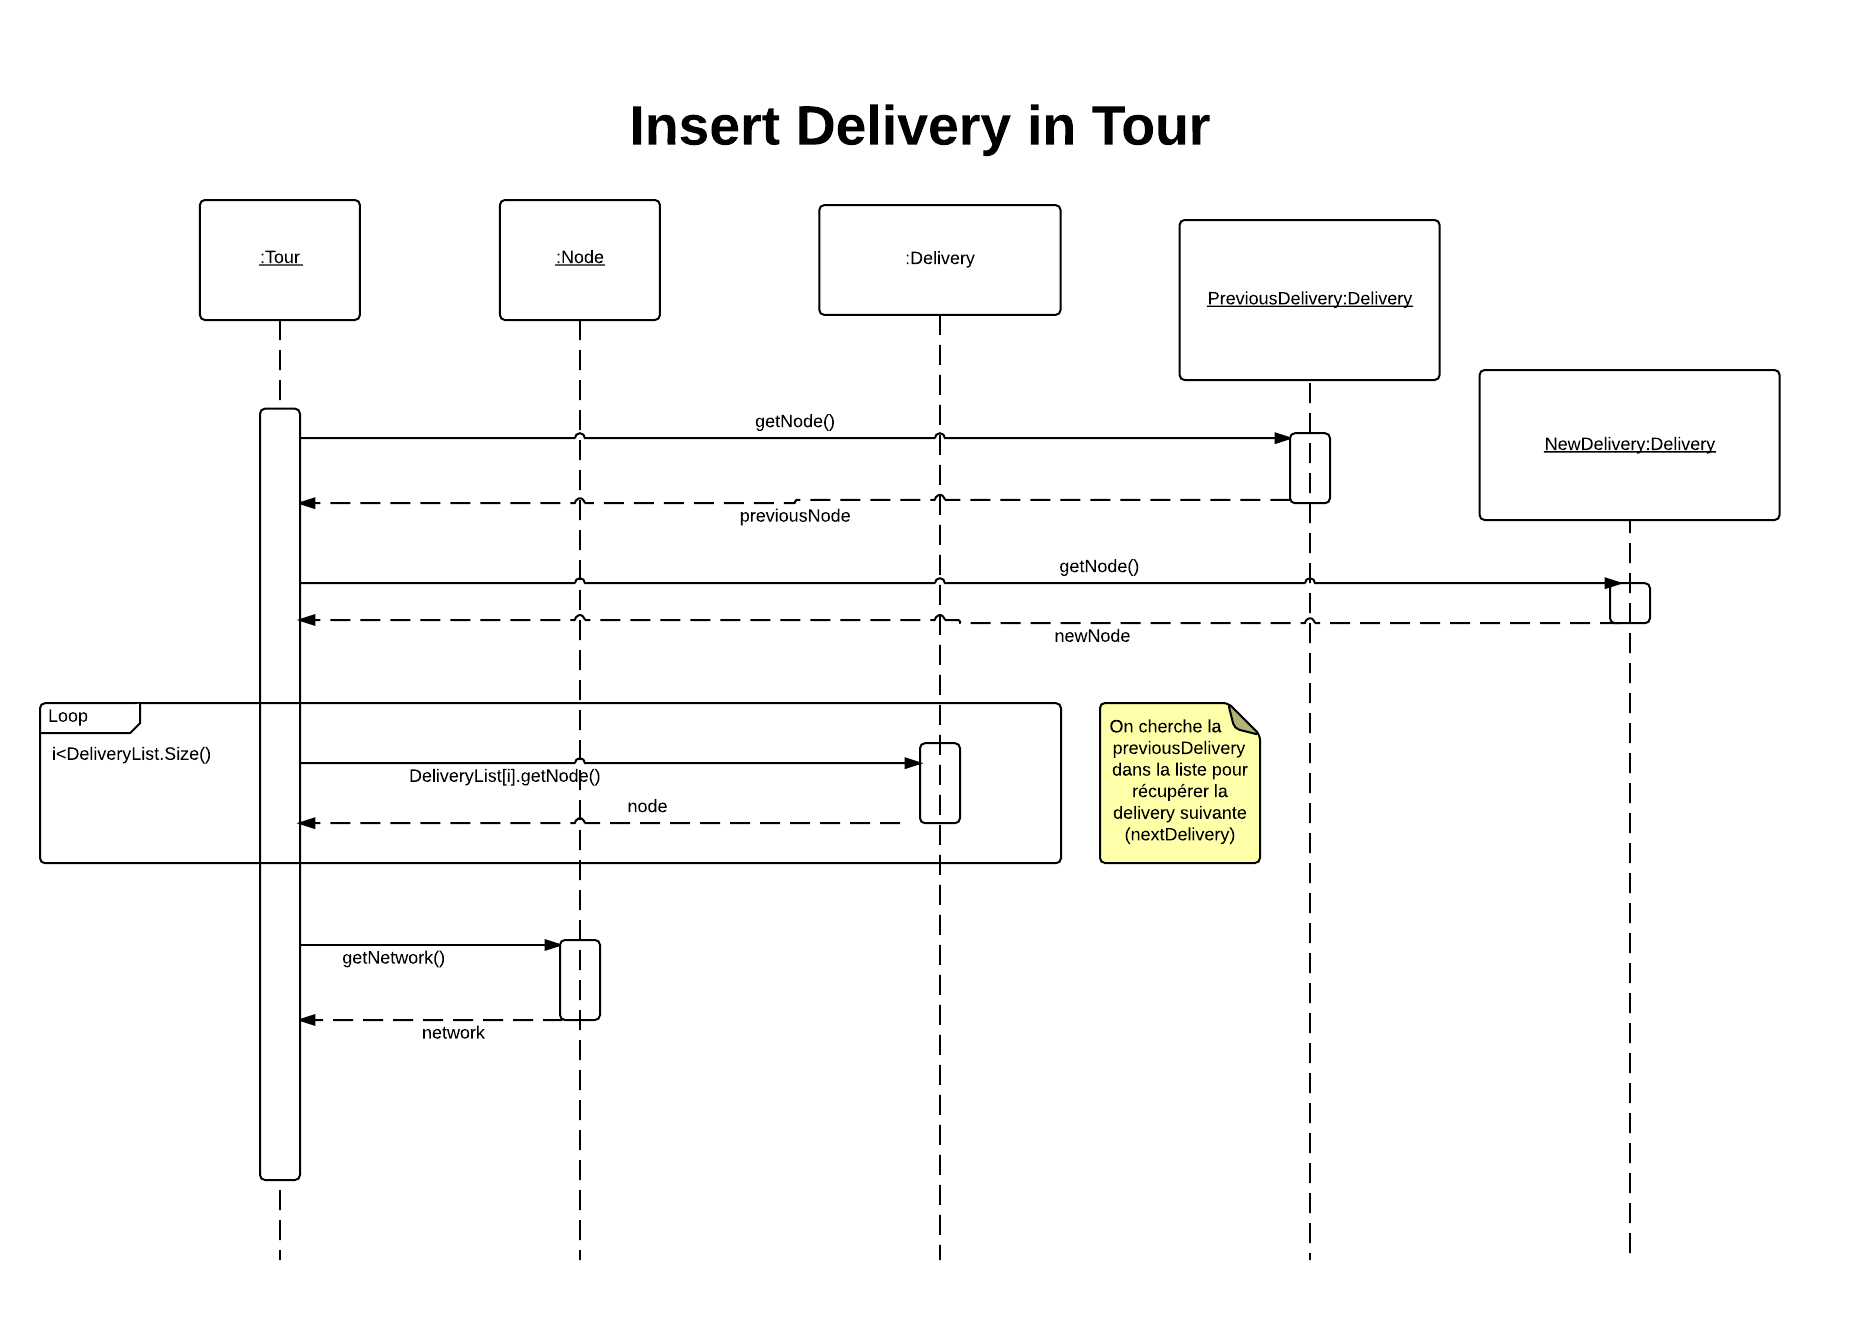
\includegraphics[width=\textwidth,height=\textheight,keepaspectratio, angle=90]{Figures/ajout_livraison5}
		\rule{35em}{0.5pt}
	\caption[Insertion d'une livraison dans la tournée]{Insertion d'une livraison dans la tournée}
\end{figure}


\begin{figure}[H]
	\centering
		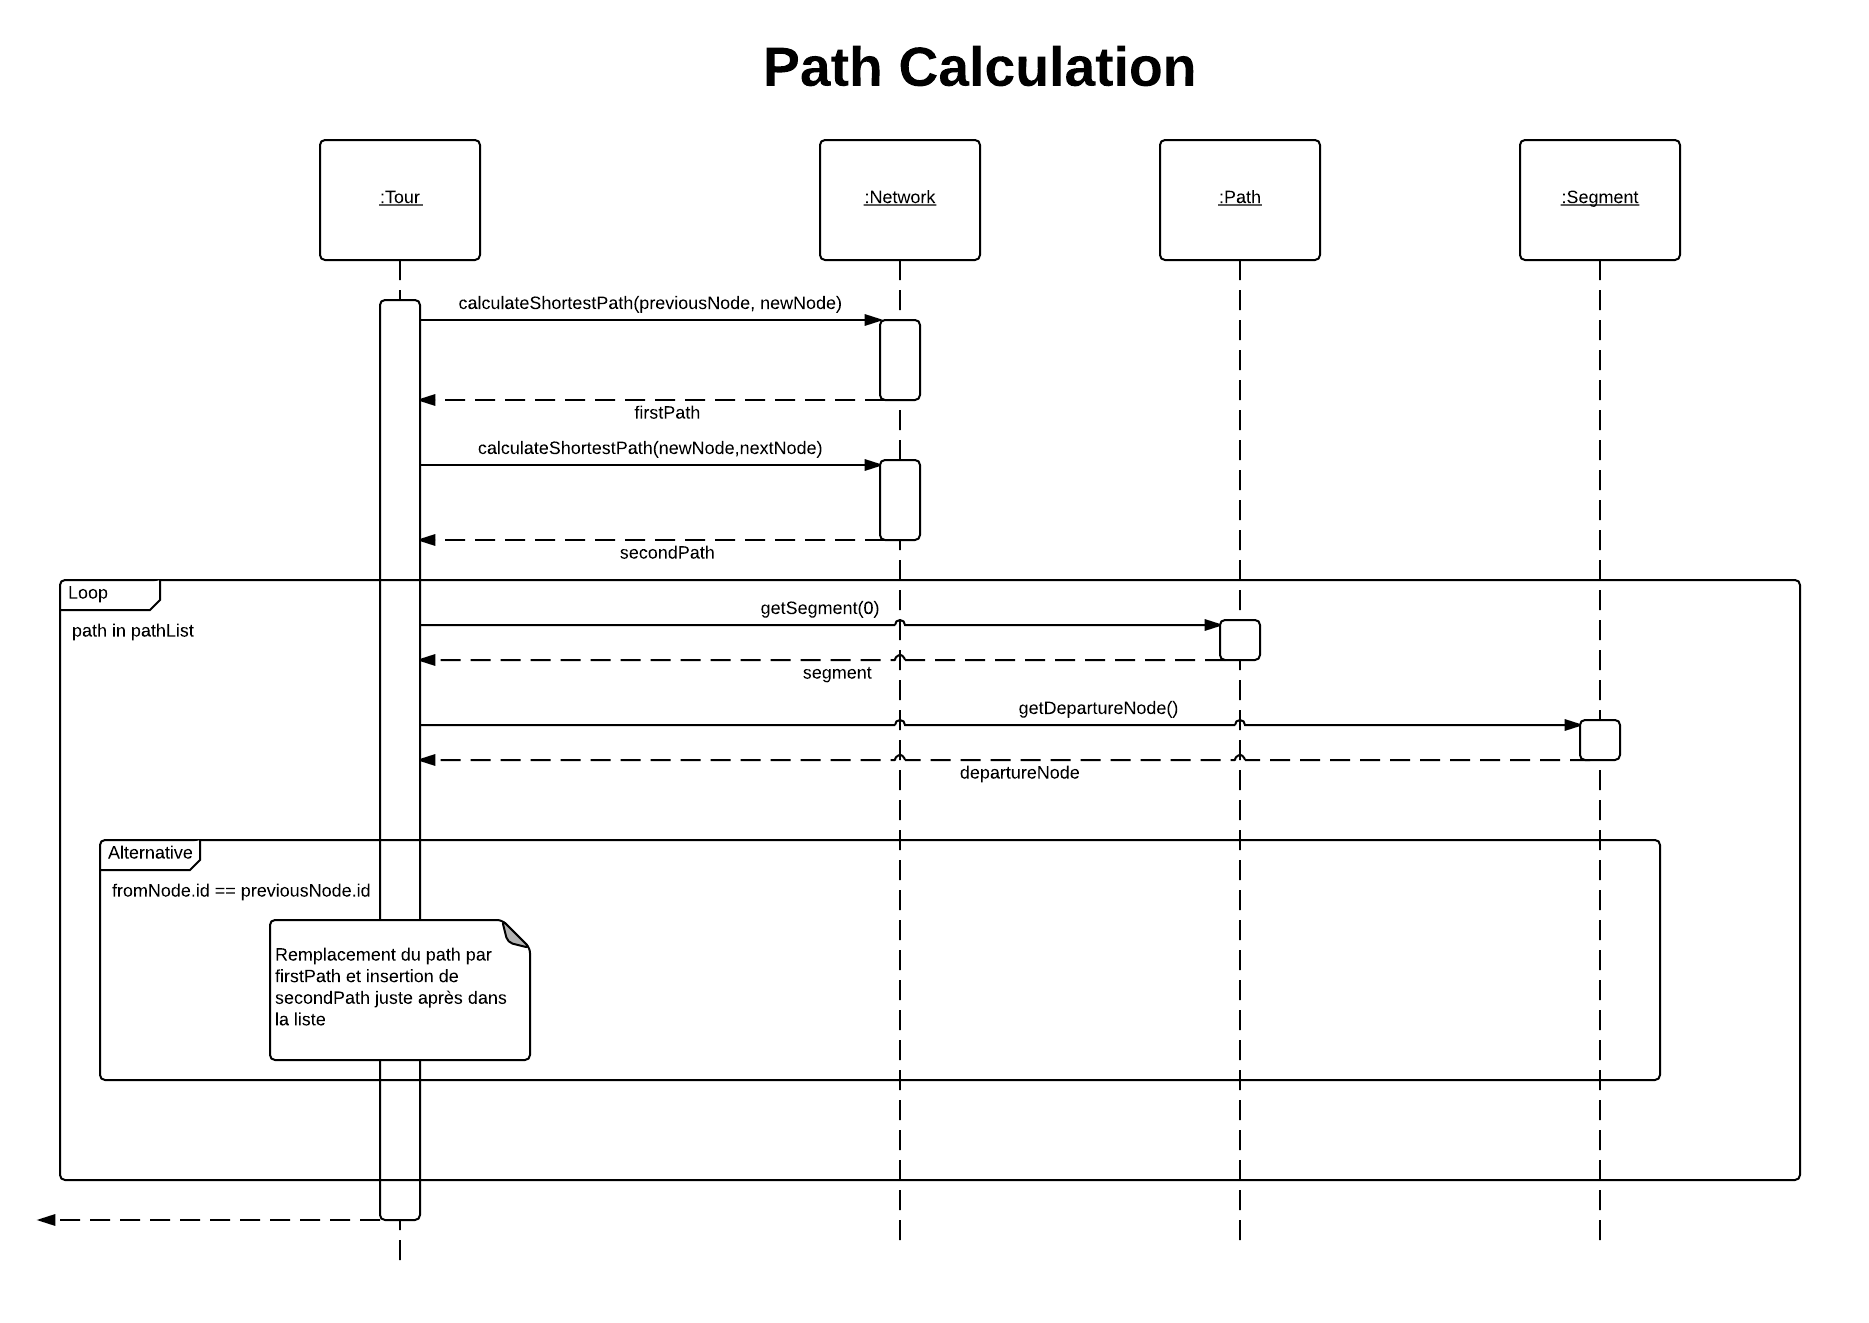
\includegraphics[width=\textwidth,height=\textheight,keepaspectratio, angle=90]{Figures/ajout_livraison6}
		\rule{35em}{0.5pt}
	\caption[Calcul du plus court chemin]{Calcul du plus court chemin}
\end{figure}

\begin{figure}[H]
	\centering
		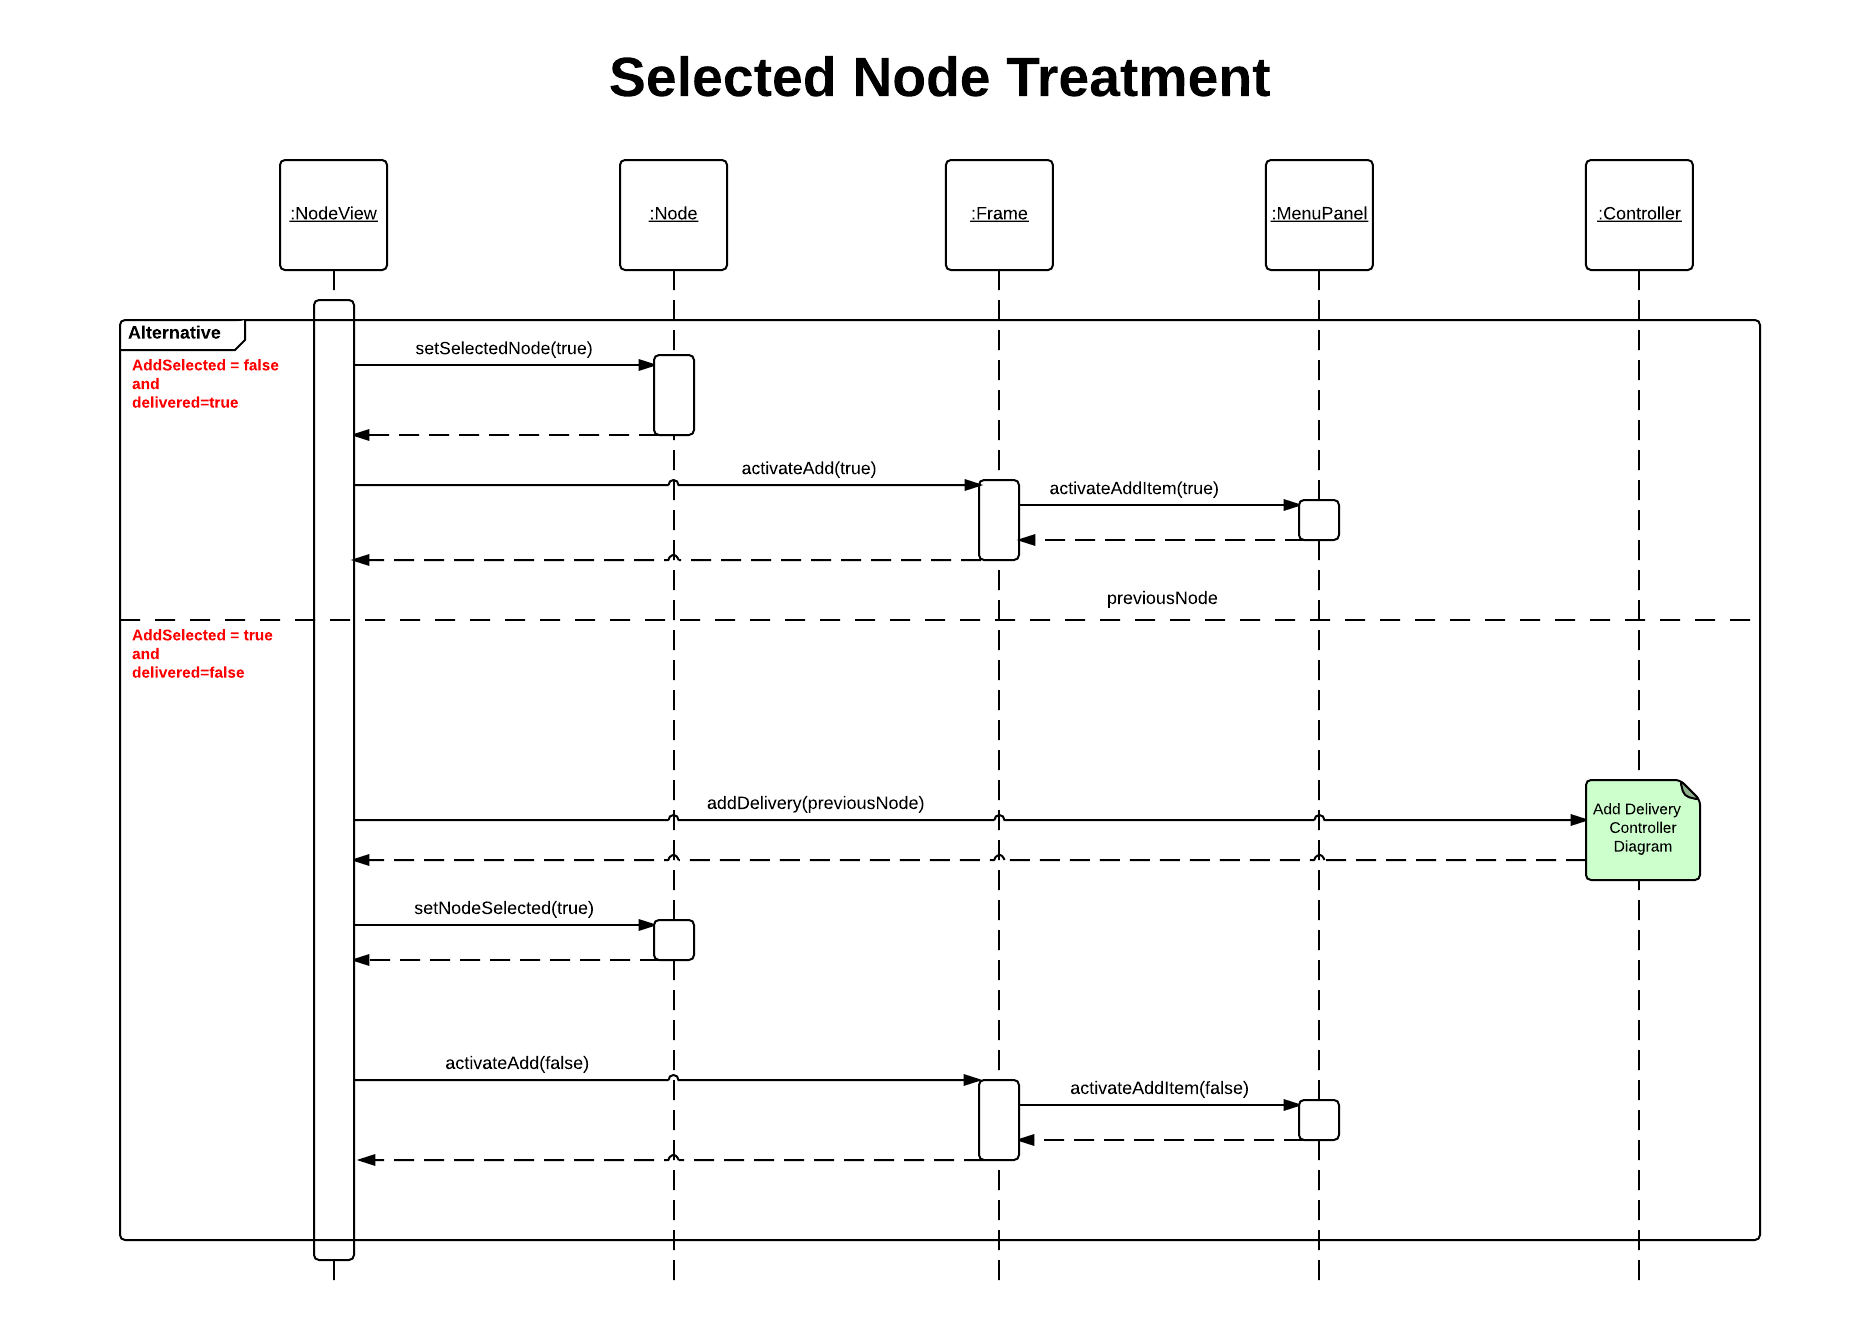
\includegraphics[width=\textwidth,height=\textheight,keepaspectratio, angle=90]{Figures/ajout_livraison7}
		\rule{35em}{0.5pt}
	\caption[Traitement du nœud sélectionné]{Traitement du nœud sélectionné}
\end{figure}
 
% Chapter Template

\chapter{Implémentation} % Main chapter title

\label{Chapter3} % Change X to a consecutive number; for referencing this chapter elsewhere, use \ref{ChapterX}

\lhead{Chapitre 3. \emph{Implémentation}} % Change X to a consecutive number; this is for the header on each page - perhaps a shortened title

%----------------------------------------------------------------------------------------
%	SECTION 1
%----------------------------------------------------------------------------------------

\section{Diagrammes de packages et de classes rétro-générés}

\subsection{Architecture générale}
\begin{figure}[H]
	\centering
		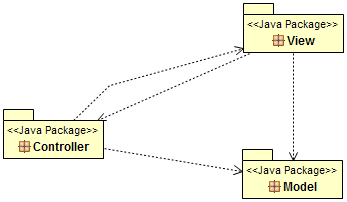
\includegraphics{Figures/retro_archi}
		\rule{35em}{0.5pt}
	\caption[Vue générale de l'application]{Vue générale de l'application}
\end{figure}

\subsection{Package model}
\subsubsection{Diagramme de classes rétro-générés}
\begin{figure}[H]
	\centering
		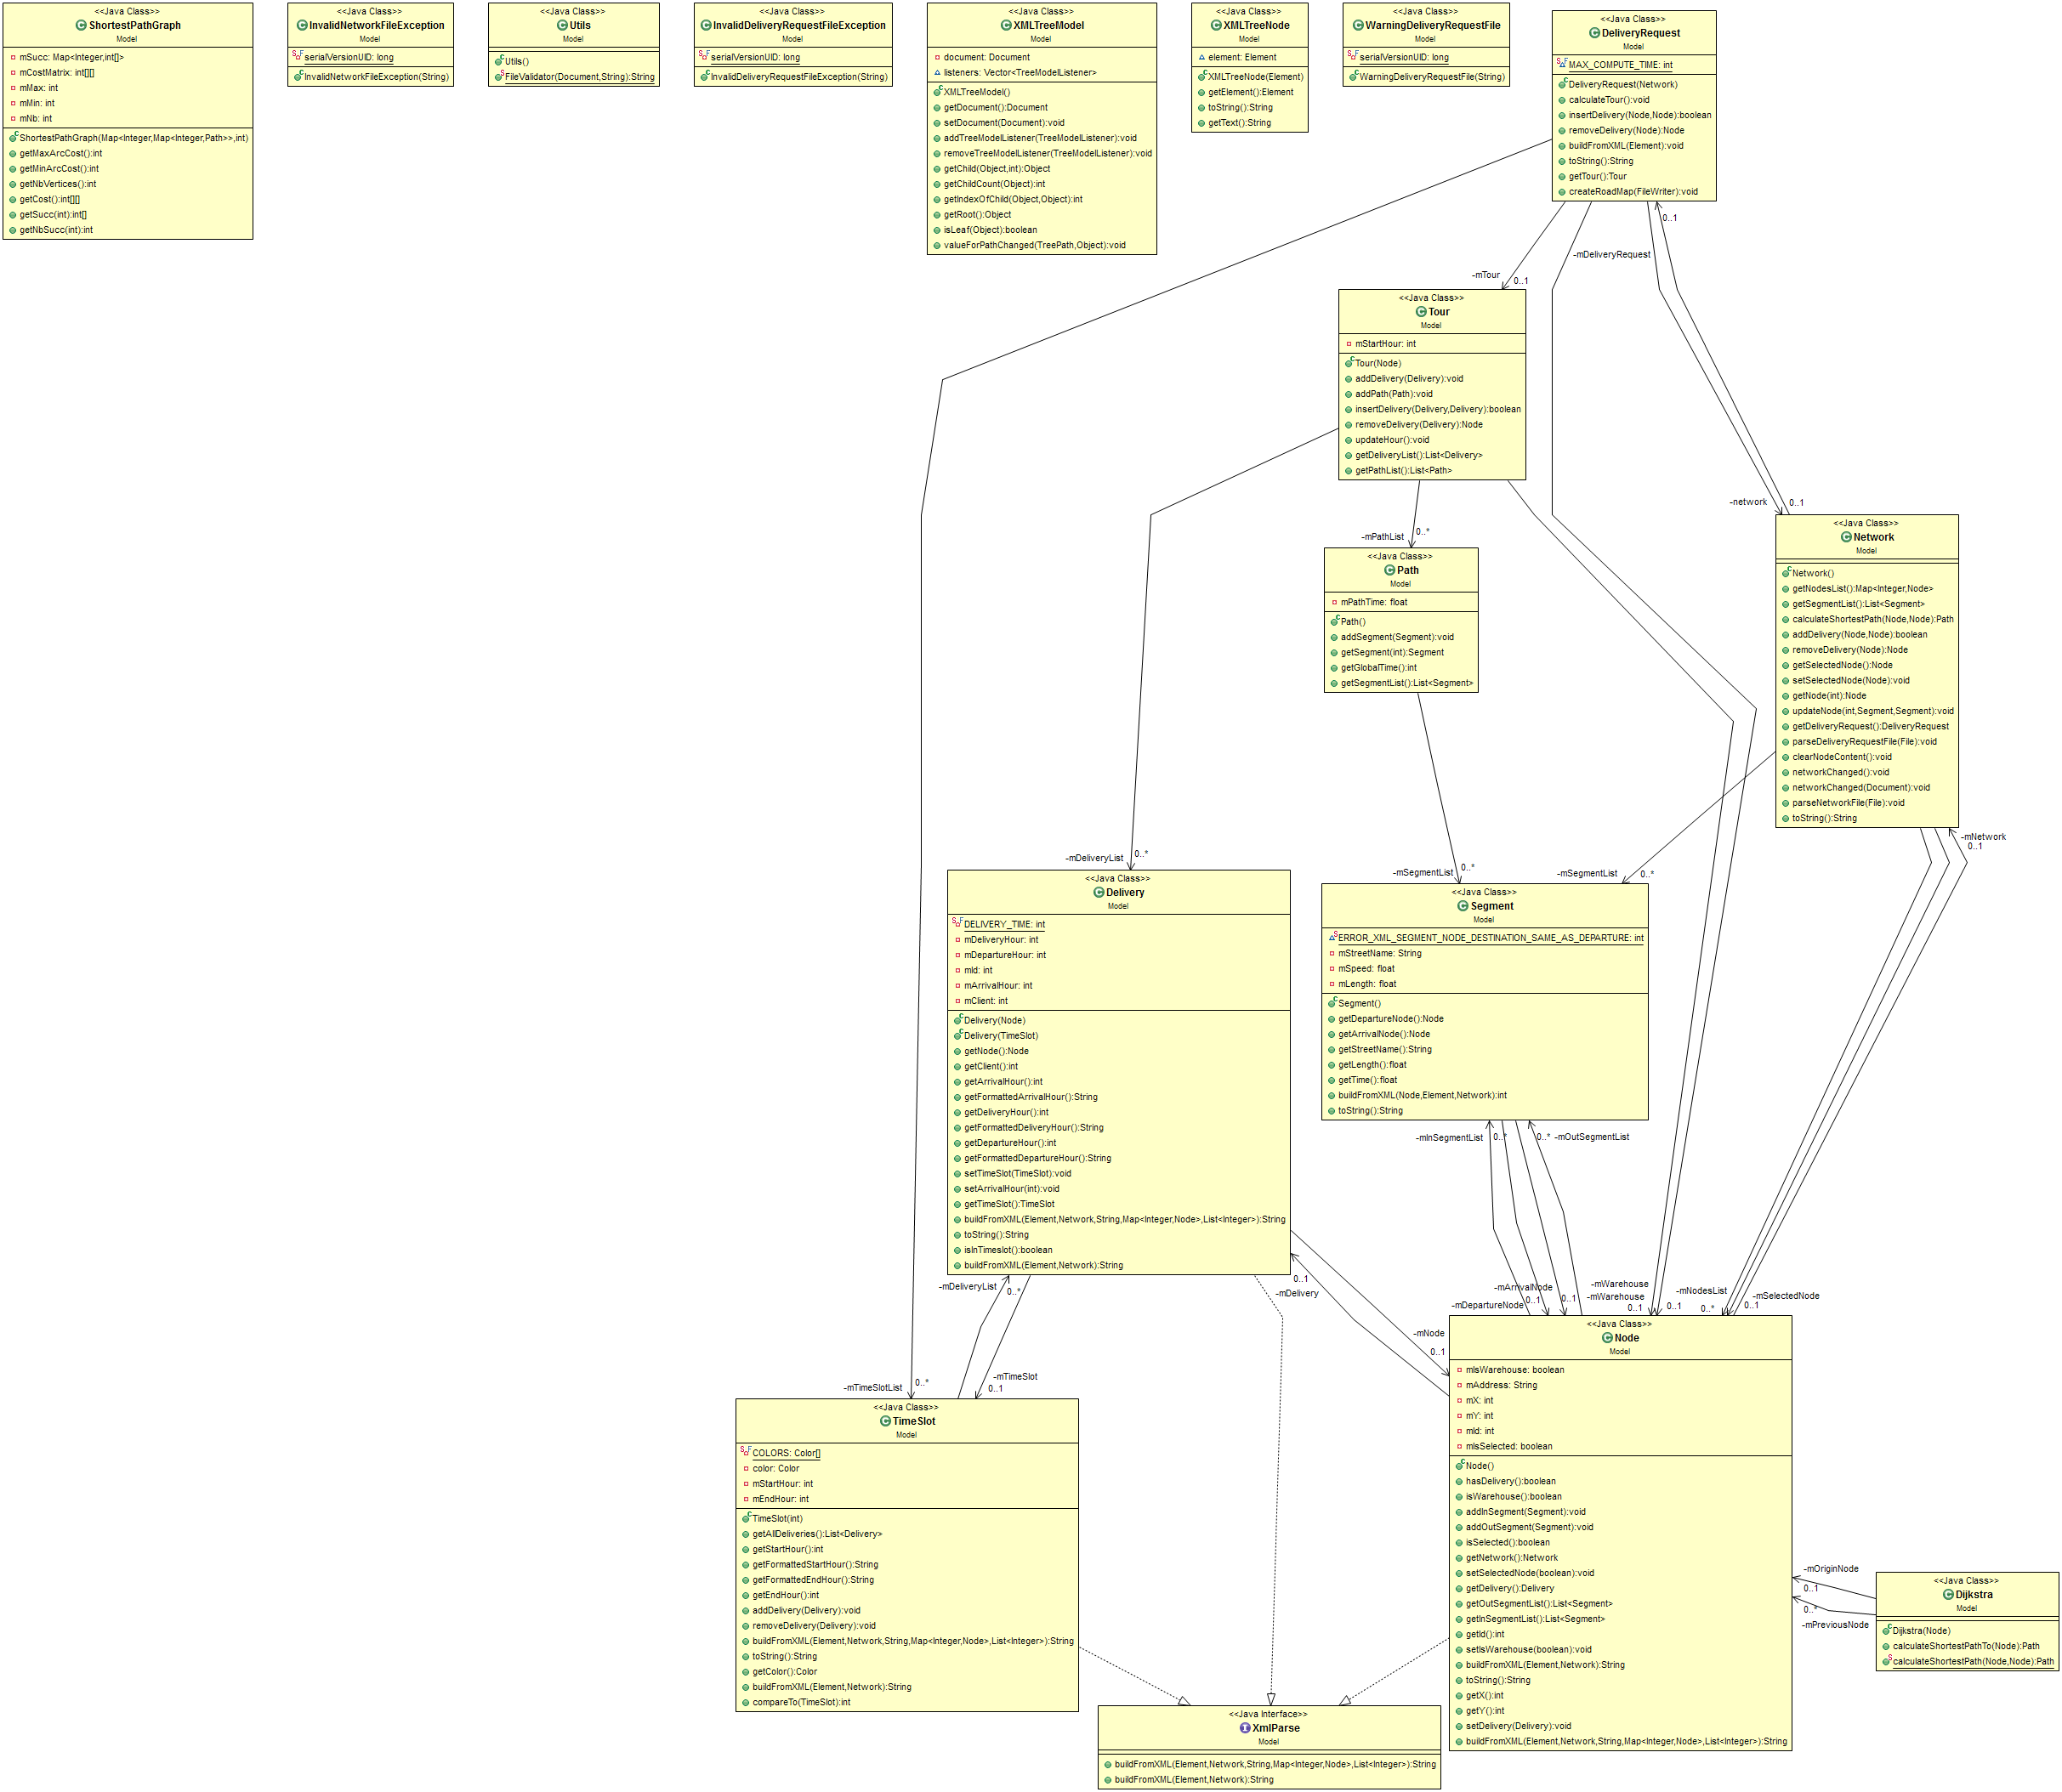
\includegraphics[width=\textwidth,height=\textheight,keepaspectratio]{Figures/retro_model}
		\rule{35em}{0.5pt}
	\caption[Diagramme de classes du package model]{Diagramme de classes du package model}
\end{figure}
\subsubsection{Dépendances}
\begin{figure}[H]
	\centering
		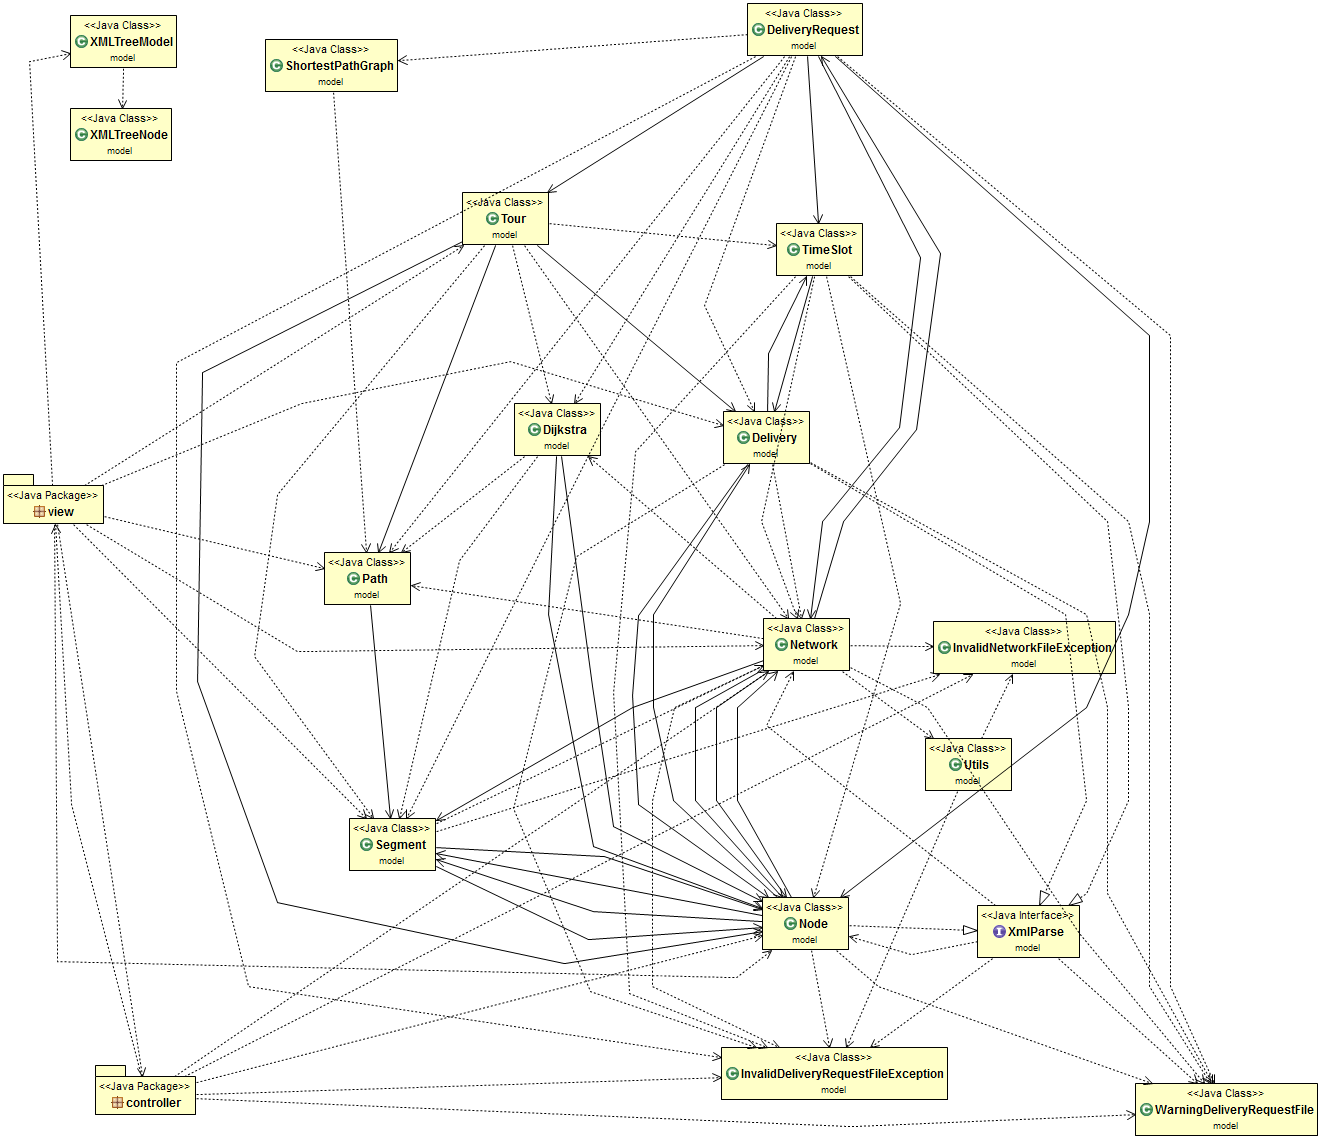
\includegraphics[width=\textwidth,height=\textheight,keepaspectratio]{Figures/retro_model_dep}
		\rule{35em}{0.5pt}
	\caption[Dépendances du package model]{Dépendances du package model}
\end{figure}

\subsection{Package view}
\subsubsection{Diagramme de classes rétro-générés}
\begin{figure}[H]
	\centering
		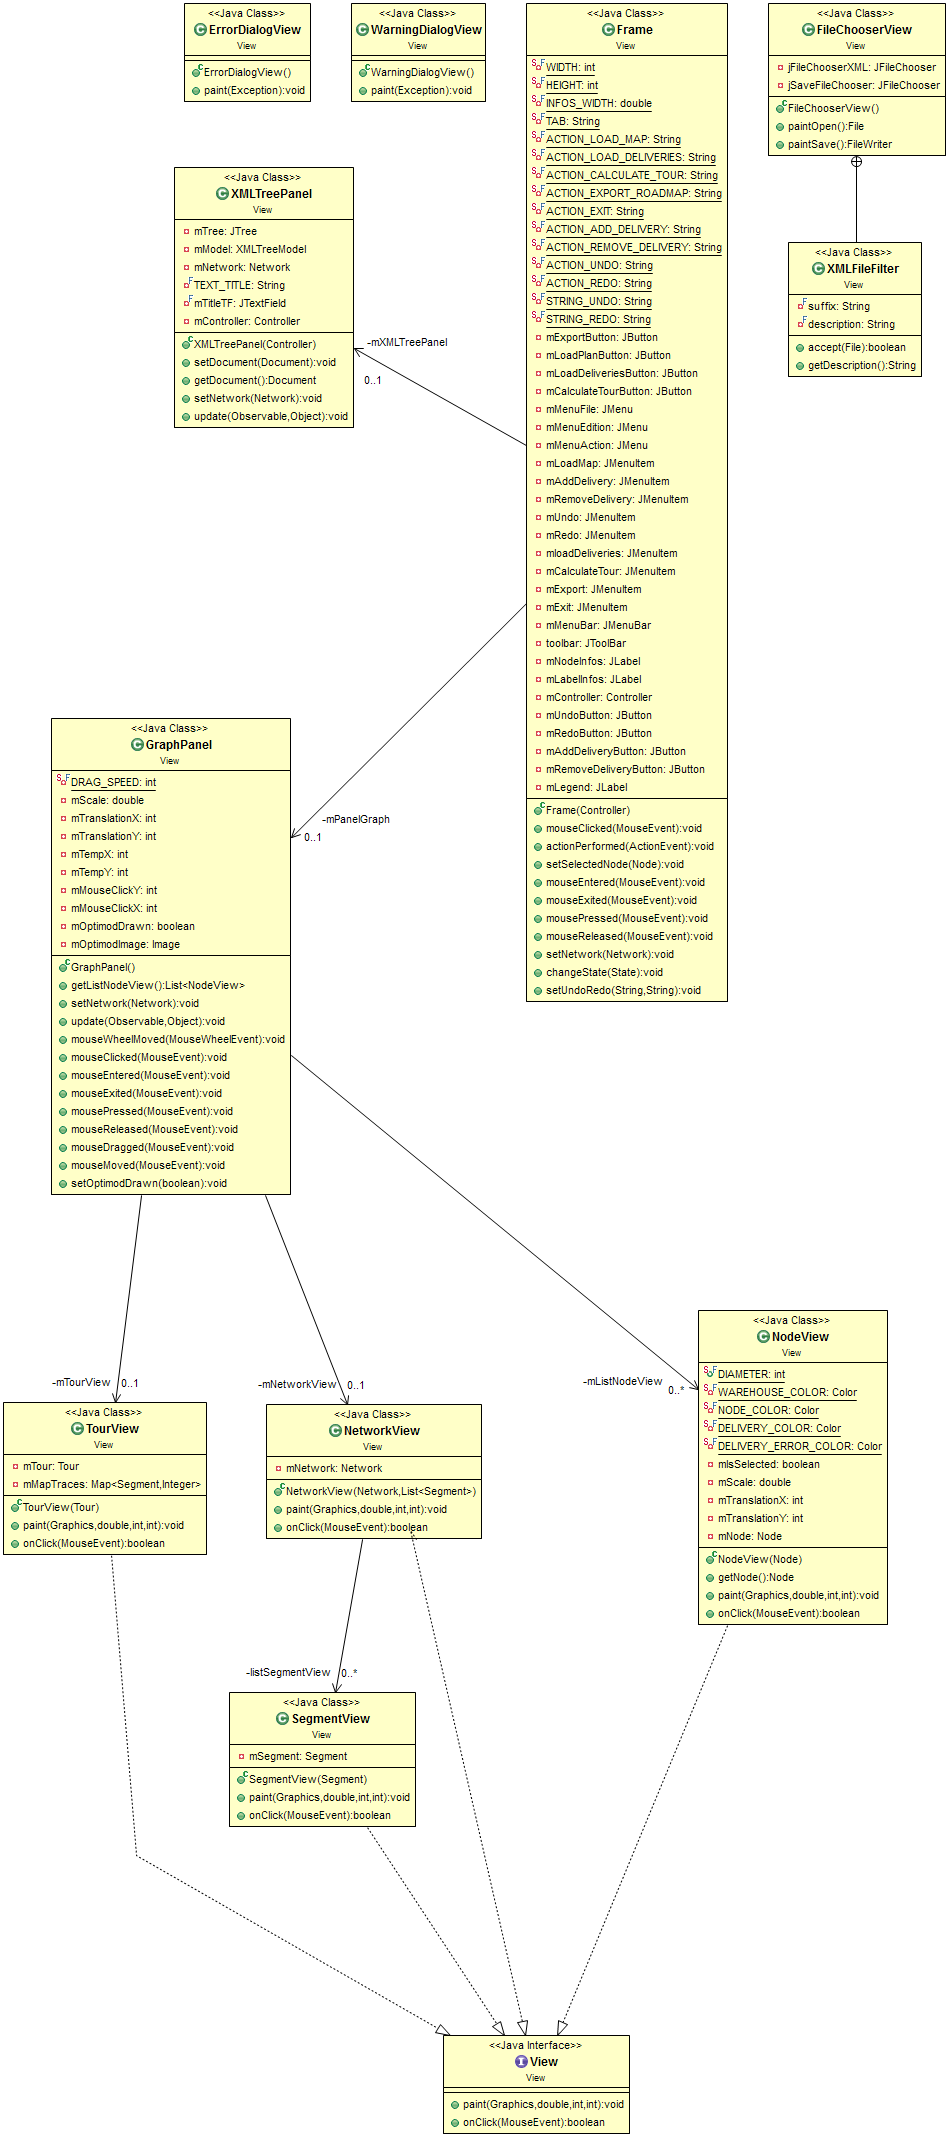
\includegraphics[width=\textwidth,height=\textheight,keepaspectratio]{Figures/retro_view}
		\rule{35em}{0.5pt}
	\caption[Diagramme de classes du package view]{Diagramme de classes du package view}
\end{figure}
\subsubsection{Dépendances}

\begin{figure}[H]
	\centering
		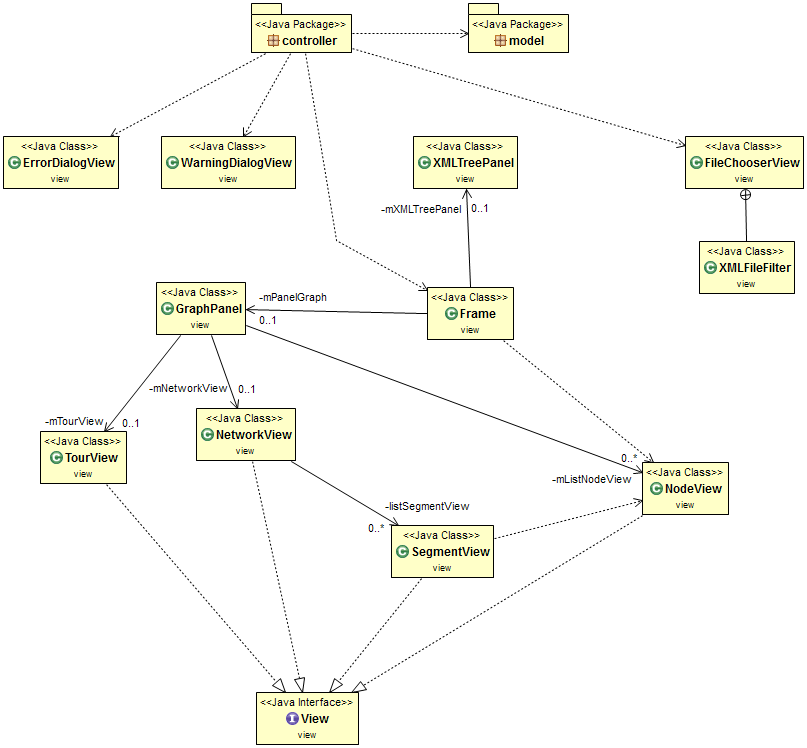
\includegraphics[width=\textwidth,height=\textheight,keepaspectratio]{Figures/retro_view_dep}
		\rule{35em}{0.5pt}
	\caption[Dépendances du package view]{Dépendances du package view}
\end{figure}
\subsubsection{Évolutions lors de l'implémentation}
Nous avons du revenir sur nos choix faits lors de la création des diagrammes de séquence pour l’ajout d’une livraison. Certains changements sont du au fait que nous avons finalement décidé d’implémenter le design pattern State pour une meilleure gestion des boutons à activer dans la fenêtre. Nous avons aussi décidé de rajouter une classe Invoker pour que la gestion des piles de commandes soit séparée du controleur. Nous avons aussi décidé d’ajouter un attribut selectedNode au Network pour éviter d’avoir à parcourir trop souvent la liste des noeuds du 
réseaux pour trouver celui qui est sélectionné. Un autre point important auquel nous n’avions pas pensé lors de la conception est l’ajout où le suppression de livraisons avec l’entrepôt juste avant ou après. En effet, l’entrepôt n’étant pas dans la liste des livraisons, il s’agit d’un cas particulier. Enfin nous avons modifié la méthode onClick pour qu’elle se contente d’indiquer si le noeud est sélectionné ou non car nous avons pensé qu’il était plus propre de lancer le reste du traitement à partir de la Frame.

\subsection{Package controller}
\subsubsection{Diagramme de classes rétro-générés}
\begin{figure}[H]
	\centering
		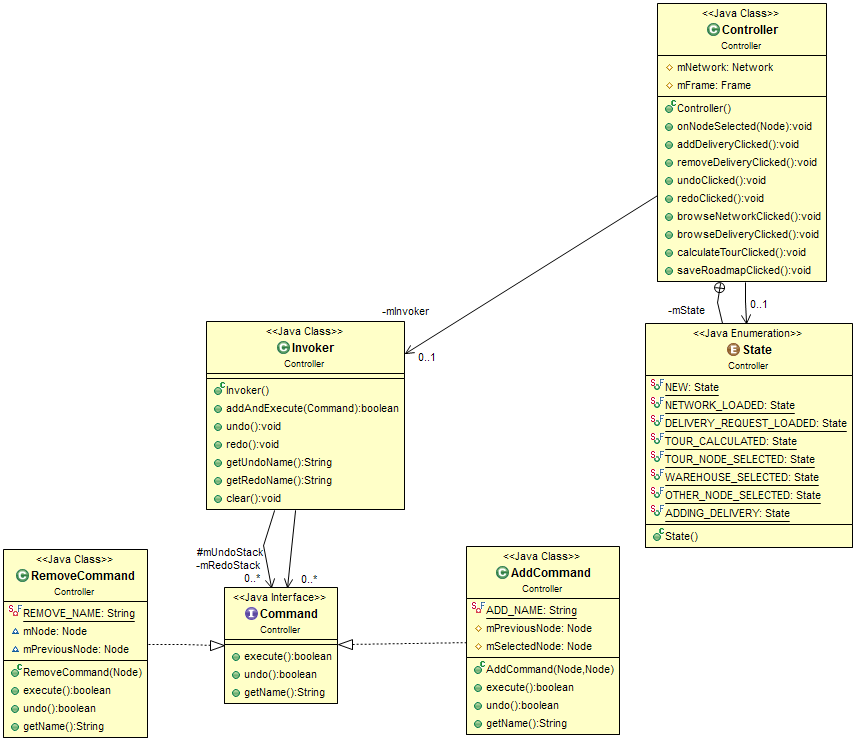
\includegraphics[width=\textwidth,height=\textheight,keepaspectratio]{Figures/retro_controller}
		\rule{35em}{0.5pt}
	\caption[Diagramme de classes du package controller]{Diagramme de classes du package controller}
\end{figure}
\subsubsection{Dépendances}

\begin{figure}[H]
	\centering
		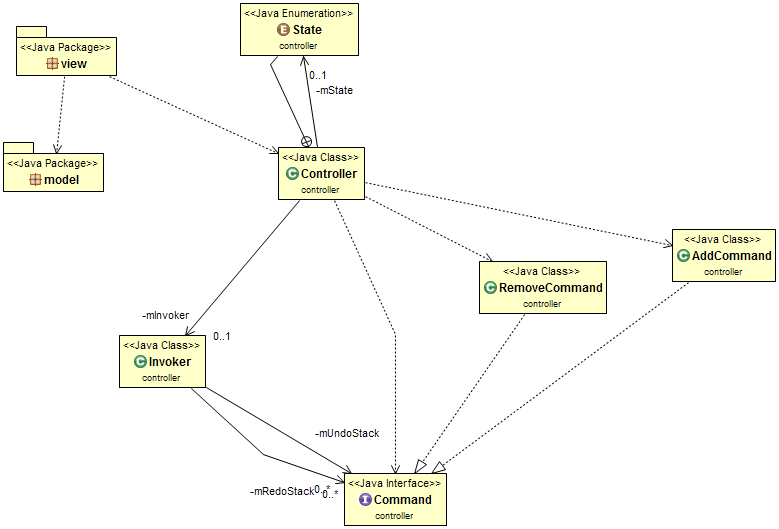
\includegraphics[width=\textwidth,height=\textheight,keepaspectratio]{Figures/retro_controller_dep}
		\rule{35em}{0.5pt}
	\caption[Dépendances du package controller]{Dépendances du package controller}
\end{figure}


%----------------------------------------------------------------------------------------
%	SECTION 2
%----------------------------------------------------------------------------------------

\section{Captures d'écran de l'application}
\begin{figure}[H]
	\centering
		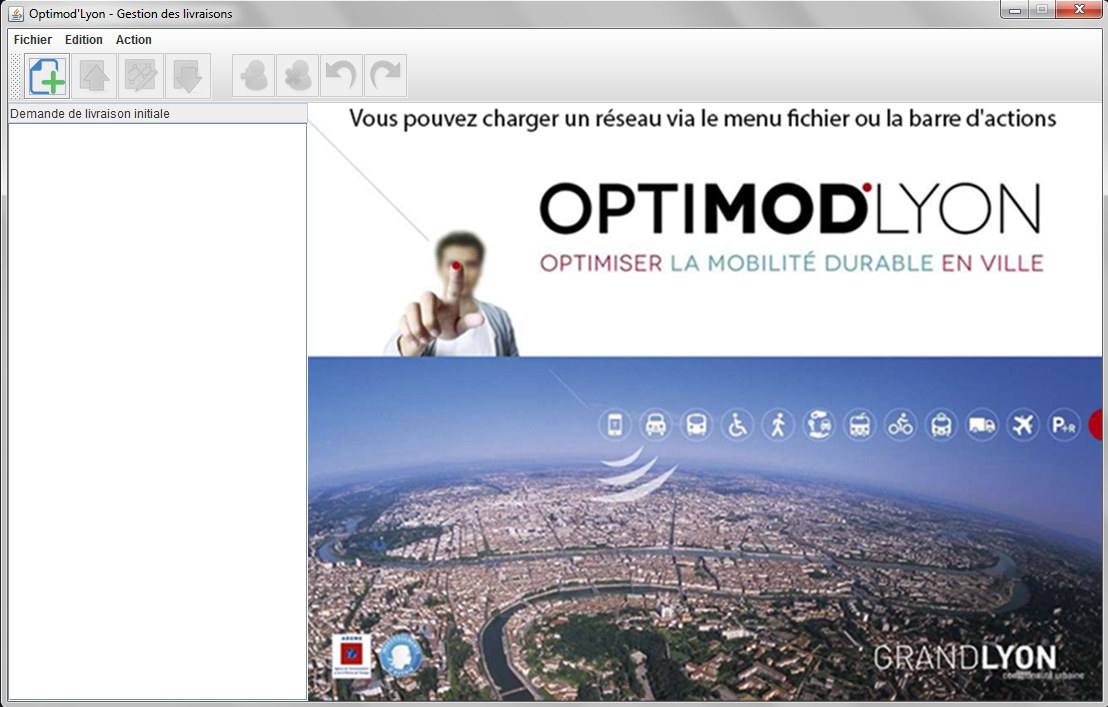
\includegraphics{Figures/welcome}
		\rule{35em}{0.5pt}
	\caption[Fenêtre d'accueil de l'application]{Fenêtre d'accueil de l'application}
\end{figure}
\begin{figure}[H]
	\centering
		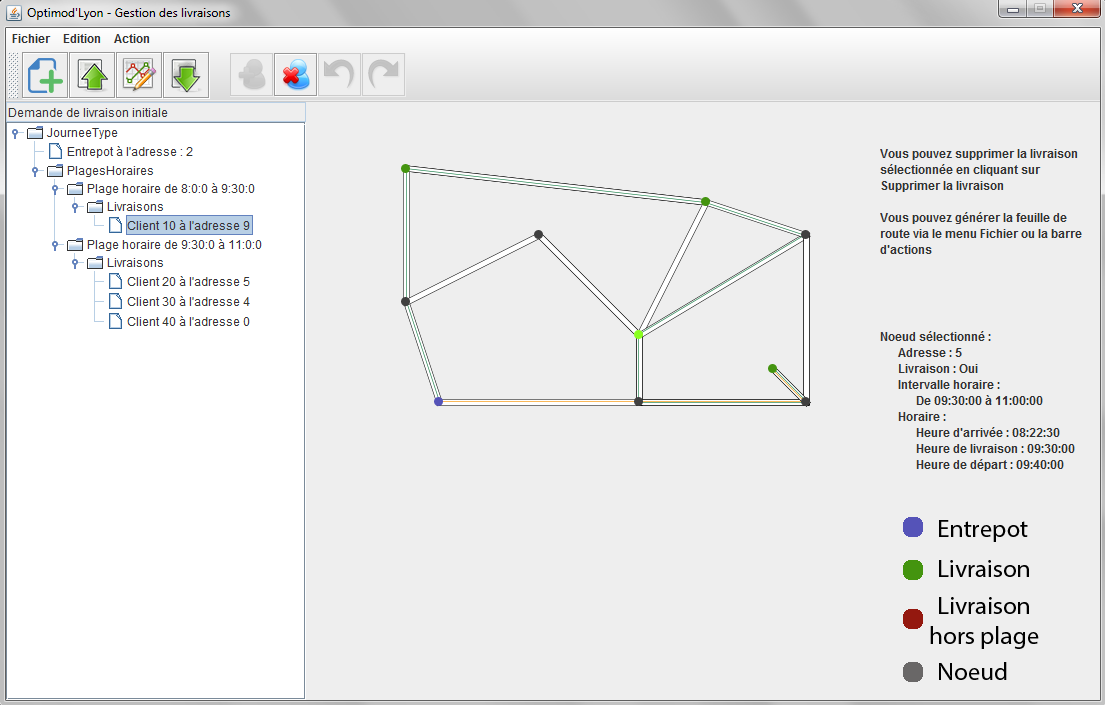
\includegraphics{Figures/plan}
		\rule{35em}{0.5pt}
	\caption[Visualisation du plan d'une zone géographique]{Visualisation du plan d'une zone géographique}
\end{figure}
\begin{figure}[H]
	\centering
		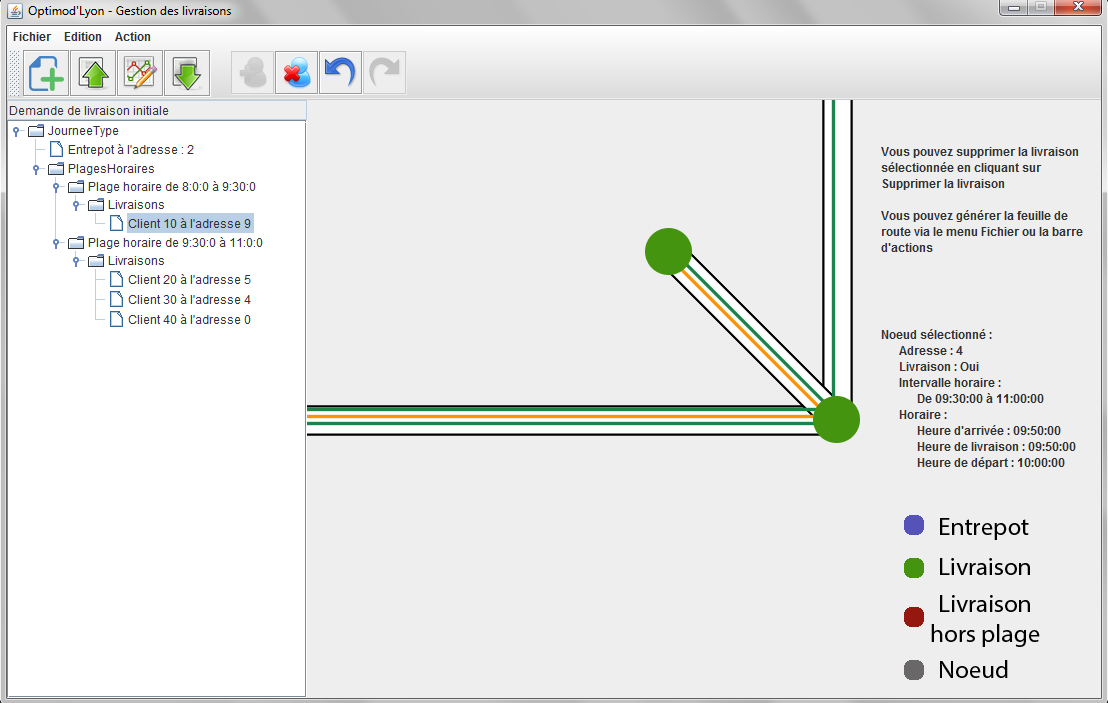
\includegraphics{Figures/path}
		\rule{35em}{0.5pt}
	\caption[Superposition d'itinéraires]{Superposition d'itinéraires}
\end{figure}
% Chapter Template

\chapter{Bilan} % Main chapter title

\label{Chapter4} % Change X to a consecutive number; for referencing this chapter elsewhere, use \ref{ChapterX}

\lhead{Chapter X. \emph{Chapter Title Here}} % Change X to a consecutive number; this is for the header on each page - perhaps a shortened title

%----------------------------------------------------------------------------------------
%	SECTION 1
%----------------------------------------------------------------------------------------

\section{Main Section 1}

Lorem ipsum dolor sit amet, consectetur adipiscing elit. Aliquam ultricies lacinia euismod. Nam tempus risus in dolor rhoncus in interdum enim tincidunt. Donec vel nunc neque. In condimentum ullamcorper quam non consequat. Fusce sagittis tempor feugiat. Fusce magna erat, molestie eu convallis ut, tempus sed arcu. Quisque molestie, ante a tincidunt ullamcorper, sapien enim dignissim lacus, in semper nibh erat lobortis purus. Integer dapibus ligula ac risus convallis pellentesque.

%-----------------------------------
%	SUBSECTION 1
%-----------------------------------
\subsection{Subsection 1}

Nunc posuere quam at lectus tristique eu ultrices augue venenatis. Vestibulum ante ipsum primis in faucibus orci luctus et ultrices posuere cubilia Curae; Aliquam erat volutpat. Vivamus sodales tortor eget quam adipiscing in vulputate ante ullamcorper. Sed eros ante, lacinia et sollicitudin et, aliquam sit amet augue. In hac habitasse platea dictumst.

%-----------------------------------
%	SUBSECTION 2
%-----------------------------------

\subsection{Subsection 2}
Morbi rutrum odio eget arcu adipiscing sodales. Aenean et purus a est pulvinar pellentesque. Cras in elit neque, quis varius elit. Phasellus fringilla, nibh eu tempus venenatis, dolor elit posuere quam, quis adipiscing urna leo nec orci. Sed nec nulla auctor odio aliquet consequat. Ut nec nulla in ante ullamcorper aliquam at sed dolor. Phasellus fermentum magna in augue gravida cursus. Cras sed pretium lorem. Pellentesque eget ornare odio. Proin accumsan, massa viverra cursus pharetra, ipsum nisi lobortis velit, a malesuada dolor lorem eu neque.

\subsection{Figures}

There will hopefully be many figures in your thesis (that should be placed in the `Figures' folder). The way to insert figures into your thesis is to use a code template like this:
\begin{verbatim}
\begin{figure}[htbp]
  \centering
    
\includegraphics{Figures/Electron.pdf}
    \rule{35em}{0.5pt}
  \caption[An Electron]{An electron (artist's impression).}
  \label{fig:Electron}
\end{figure}
\end{verbatim}
Also look in the source file. Putting this code into the source file produces the picture of the electron that you can see in the figure below.

\begin{figure}[htbp]
	\centering
		
\includegraphics{Figures/Electron.pdf}
		\rule{35em}{0.5pt}
	\caption[An Electron]{An electron (artist's impression).}
	\label{fig:Electron}
\end{figure}

%----------------------------------------------------------------------------------------
%	SECTION 2
%----------------------------------------------------------------------------------------

\section{Main Section 2}

Sed ullamcorper quam eu nisl interdum at interdum enim egestas. Aliquam placerat justo sed lectus lobortis ut porta nisl porttitor. Vestibulum mi dolor, lacinia molestie gravida at, tempus vitae ligula. Donec eget quam sapien, in viverra eros. Donec pellentesque justo a massa fringilla non vestibulum metus vestibulum. Vestibulum in orci quis felis tempor lacinia. Vivamus ornare ultrices facilisis. Ut hendrerit volutpat vulputate. Morbi condimentum venenatis augue, id porta ipsum vulputate in. Curabitur luctus tempus justo. Vestibulum risus lectus, adipiscing nec condimentum quis, condimentum nec nisl. Aliquam dictum sagittis velit sed iaculis. Morbi tristique augue sit amet nulla pulvinar id facilisis ligula mollis. Nam elit libero, tincidunt ut aliquam at, molestie in quam. Aenean rhoncus vehicula hendrerit.
\chapter*{Glossaire}
\addcontentsline{toc}{chapter}{Glossaire}
\begin{description}
\item [Jour]De 0:00 à 23:59
\item [Feuille de route (roadMap)]Tournée validée et imprimée en version papier
\item [Tournée (Tour)]Itinéraire associé avec les horaires de passage pour chaque \item [livraison] (départ + arrivée)
\item [Demande de livraisons (Delivery Request)] Ensemble de livraisons à programmer un jour donné 
\item [Heure (Delivery Hour)]Heure de passage chez un client
\item [Livraison (Delivery)]Action de déposer un colis à une heure et une adresse données
\item [Zone géographique]Ensemble de noeuds proches géographiquement
\item [Livreur]Personne qui effectue les livraisons
\item [Plage horaire (TimeSlot)] Intervalle de temps (hh:mm - hh:mm)  dans lequel la livraison est prévue
\item [Itinéraire]Parcours de l’entrepôt à l’entrepôt en passant dans l’ordre par des points de livraison mais sans horaires associés au aux livraisons
\item [Réseau (Network)]Plan global de l’agglomération
\item [Tronçon de route (Segment)]Route reliant deux points contigüs dans le graphe sans passer par d’autres points (élément unitaire de route) ~ arc du graphe    
\item [Chemin (Path)]Succession de tronçons
\item [Noeud (Node)]Point sur le graphe (potentiellement livrable)
\item [Cadres]Différentes zones contenues dans une fenêtre de l’IHM
\end{description} 

%----------------------------------------------------------------------------------------
%	THESIS CONTENT - APPENDICES
%----------------------------------------------------------------------------------------

\addtocontents{toc}{\vspace{2em}} % Add a gap in the Contents, for aesthetics

%\appendix % Cue to tell LaTeX that the following 'chapters' are Appendices

% Include the appendices of the thesis as separate files from the Appendices folder
% Uncomment the lines as you write the Appendices

%% Appendix A

\chapter{Appendix Title Here} % Main appendix title

\label{AppendixA} % For referencing this appendix elsewhere, use \ref{AppendixA}

\lhead{Appendix A. \emph{Appendix Title Here}} % This is for the header on each page - perhaps a shortened title

Write your Appendix content here.
%\input{Appendices/AppendixB}
%\input{Appendices/AppendixC}

\addtocontents{toc}{\vspace{2em}} % Add a gap in the Contents, for aesthetics

\backmatter

\end{document}